\documentclass{article}
\usepackage[margin=1in]{geometry}
\usepackage{amsmath,amsfonts}
\usepackage{listings}
\usepackage{color}
\usepackage{verbatim}
\usepackage{graphicx}
\usepackage{float}
\usepackage{pdfpages}\usepackage[section]{placeins}
\usepackage{tikz}
\usetikzlibrary{backgrounds}

\definecolor{dkgreen}{rgb}{0,0.6,0}
\definecolor{gray}{rgb}{0.5,0.5,0.5}
\definecolor{mauve}{rgb}{0.58,0,0.82}
\definecolor{black}{rgb}{0,0,0}

\title{\textsc{\textbf{Engineering and Design Journal}}}
\author{\textsc{FTC Team 4278 {\color{dkgreen}de.evolution}}}
\date{}

\renewcommand{\abstractname}{Introduction}

\lstset{frame=tb,
  language=C++,
  aboveskip=3mm,
  belowskip=3mm,
  showstringspaces=false,
  basicstyle={\small\ttfamily},
  numbers=none,
  numberstyle=\tiny\color{gray},
  keywordstyle=\color{blue},
  commentstyle=\color{dkgreen},
  stringstyle=\color{mauve},
  breaklines=true,
  breakatwhitespace=true
  tabsize=2
}

\makeatletter

\tikzset{%
  fancy quotes/.style={
    text width=\fq@width pt,
    align=justify,
    inner sep=1em,
    anchor=north west,
    minimum width=\textwidth,
  },
  fancy quotes width/.initial={.8\textwidth},
  fancy quotes marks/.style={
    scale=6,
    text=black,
    inner sep=0pt,
  },
  fancy quotes opening/.style={
    fancy quotes marks,
  },
  fancy quotes closing/.style={
    fancy quotes marks,
  },
  fancy quotes background/.style={
    show background rectangle,
    inner frame xsep=0pt,
    background rectangle/.style={
      fill=gray!25,
      rounded corners,
    },
  }
}

\newenvironment{fancyquotes}[1][]{%
\noindent
\tikzpicture[fancy quotes background]
\node[fancy quotes opening,anchor=north west] (fq@ul) at (0,0) {``};
\tikz@scan@one@point\pgfutil@firstofone(fq@ul.east)
\pgfmathsetmacro{\fq@width}{\textwidth - 2*\pgf@x}
\node[fancy quotes,#1] (fq@txt) at (fq@ul.north west) \bgroup}
{\egroup;
\node[overlay,fancy quotes closing,anchor=east] at (fq@txt.south east) {''};
\endtikzpicture}

\makeatother

\begin{document}
\maketitle

\begin{fancyquotes}
Ever since last spring, when their team members did a presentation at our school for Science Discovery Day, they have been an inspiration to our robotics students and are chiefly responsible for encouraging our 8th graders to start an FTC team this year. \newline \newline
--David Warner, Coach for the RSF Eagles FTC Team
\end{fancyquotes}
\newline \newline \newline
\begin{fancyquotes}
De.evolution team members are committed to advancing understanding of robotics in
middle and high schools and to spreading the message of the excitement, team spirit and
intellectual stimulation that FIRST competitions provide.
\newline \newline
--The Rancho Santa Fe Review
\end{fancyquotes}
\newline \newline \newline
\begin{fancyquotes}
Historically, our team has been about building the best possible robot. This year,
however, the focus of our team has shifted from winning the competition to helping others
succeed, as we have realized that this, truly, is what FIRST is about.\newline\newline
The teams at the competitions are wonderful, as always. The cooperative spirit of the events is fundamentally alters one's perspective, as it grows into more than simply a competition for awards.
\newline \newline
-- Noah Sutton-Smolin, Co-president of de.evolution
\end{fancyquotes}

\newpage 
\begin{abstract}
\textbf{FTC Team 4278 proposes} the creation of a robot to address all aspects of the FTC 2013-14 competition, ``Block Party.'' The proposed design has the capacity to address, in the teleoperated period: (1) retrieval of blocks; (2) placement of blocks into the block crates; (3) raising the FTC flag; (4) hanging on the field bar. In addition, during the autonomous period, the robot will address the following elements: (1) placement of blocks in the correct bin, as indicated by an IR beacon; (2) maneuvering to the ramp. 

In order to achieve these goals, it was determined that the robot should: (1) be very difficult to push; (2) be fast and reliable in movement; (3) have a low center of gravity; (4) have as few unique components as possible; (5) be as compact as possible; (6) pick up blocks with at most one motion; (7) place blocks in crates with at most one motion; (8) hang with at most either two motions on an existing component, or one motion on a new component; (9) be able to raise the flag with one component; (10) be electrically stable, generating as little static as possible. 

Goals set for autonomous include: (1) being able to score in the crate denoted by the IR beacon; (2) being able to travel to the nearest ramp; (3) being able to address and recover from any problems which may arise on the field, including, but not limited to, obstructions caused by other robots; (4) potentially being able to score both autonomous blocks. For (3), the intent is to travel onto the ramp regardless of potential obstruction by other robots. Decision logic is used to avoid obstructions.

Over the course of this engineering document, we address these problems, determine how we solve them, and explain the process which lead to these conclusions. Most notably, the development of a prototype robot allowed us to identify critical problems with our design and address them before implementation.

The code which goes into this design will also be explained. \newline

\textbf{FTC Team 4278 also aims} to create a foundation for all FIRST teams by: (1) helping teams online and in the pits where possible; (2) promoting the philosophy that the FIRST Tech Challenge is primarily about education and secondarily about competition; (3) raising awareness about FIRST in our high school and region; (4) supporting the success of teams through the distribution of knowledge and acquired experience.

We aim to, first and foremost, help teams succeed - the competition is not genuine if teams are not operating at maximum capacity - and secondarily, spread awareness about FIRST to students everywhere to bring them into the FIRST program.

\end{abstract} \newpage\tableofcontents\newpage\setlength{\parskip}{4pt}

\section{Robot Design and History Overview}
In this section, we detail each component of the robot, the design decisions that went into it, important and critical tests, and the general development of our design.

Over the past four years, our design strategy has changed significantly. We have gone through multiple paradigm shifts in our design process. Our first year, we simply threw ourselves at the problem and left the result to be decided. This worked wonderfully, but in retrospect, much of that was simply sheer luck. We struck the correct idea, and executed it effectively, but not to the best of our ability. 
	
As a result, the second year, our effectiveness slumped slightly. Though we still won several awards for placing third in local competitions, we did not perform to our expected standard. The reasons for this are twofold: First, we failed to properly conceptualize what it is we intended to do before making an attempt at execution. In this way, the robot's design suffered significantly from problems which could have been solved with some forethought. Secondly, we failed to properly test the components of the design before implementation. We threw parts together without accurately testing each one for validity, and refused to change the parts that did not work.

We drew many lessons from that year, and in our third year, we developed a full SolidWorks model of our design, and created a defined intent for our robot before building. We prototyped several components before implementing them. We did still run into issues, but they were not issues we could necessarily have predicted or forseen over such a short timescale. All things considered, we created a highly effective robot, breaking the world record score, and scoring a maximum of over 300 points on the field by ourselves.

This year, we had to think a bit more rigorously about our design. We hearkened back to the 2011-2012 FTC Challenge, ``Bowled Over!'' during which we struggled to actually lift the balls off the ground. We recognized going into this year that pulling objects out of a dispenser is much easier to design and engineer around than lifing objects off the ground. However, in the usual spirit of our team, we wanted to do it all. When we set out to tackle this challenge, we decided we would find the IR beacon, move to the bridge, score tons of blocks, raise the flag, and hang our robot. We decided that the challenge was \textit{doable}, and we would meet its challenge. This, below, is what we have done\ldots

\subsection{General Structure and Design}
We decided very early on what the style of our robot's design would be. We recognized that it is possible to determine some components' effectiveness without actually having \textit{designed} the other compoments necessarily. 

We started with the frame structure. We decided there were a couple main approaches: we could either lift blocks straight off the ground, or drive into blocks and lift them up that way. One way supports a high, square frame with a tall clearance, and the other supports an ``A-frame,'' so called for its resemblance to a block-letter A. This would allow us to pick up blocks with the front of our robot, while still leaving plenty of room for electronics. We chose the A-frame over the square frame for sheer simplicity and potentially synergistic design with other components of the robot. 

At this time, we had imagined the flag spinning motor on the front of the robot, an arm to manipulate blocks, and various motors and errata on the sides of the robot. While we have significantly changed the vision from its original form, it is still true to these aspects in particular. We have placed a flag spinner on the front of our frame, we have an arm to manipulate blocks, and the gears are stored in the side panels. 

As optimal as we may have decided the A-frame to be, there were a few considerations to think carefully about before actual implementation. These were lessons we learned from ``Bowled Over!''. The first topic we needed to consider was stability. When we designed the frame for the challenge two years ago, we paid very little attention to stability. As a result, the weight we placed on the center of the robot caused it to cave in where it should not have. The front wheels warped inward, and the electronics came loose under tension. Additionally, the muli-segment arm had pressure in places it was not designed to support. We will reveal how we addressed this later in this section.

\subsection{Considerations for Support, Structure, and Placement}
We needed to make particular consideration for structure and weight distribution on the final design, as we had chosen a type of frame which becomes unstable if not properly constructed. We decided very early on that we would construct the robot mostly from raw materials, so the first consideration was of material. We were presented with several options, nobody on the team questioned the choice of delrin as the appropriate material.

\paragraph{Material Selection} Delrin was chosen primarily for its strength and resilience. It is an easy material to lathe and cut, both by laser and hand, and it does not damage easily. It is very strong in thick directions, and is also relatively lightweight. Tetrix aluminum frame pieces are far, far too flexible and pliable, and become warped or damaged easily during competition. Delrin does not often even so much as scratch.

Even so, we could not depend on delrin entirely. After some consideration to structure, we decided that the easiest way to prevent the side panels from caving in was to both make them thicker and support them against each other. We decided that the wheels and gears could go in between two panels, which would be spaced for stability. These would act as our gear boxes. Additionally, the two gearbox panels would be supported by the entire middle section of the robot, which would prevent them from caving in. We decided support bars would be needed across the center of the robot. This, we decided, is doable.

Standoffs were used to support the two panels of the gearboxes.

\paragraph{Center of Gravity} Some consideration had to be given to center of gravity. In deciding we wanted to use an arm, we effectively filled most of the robot with air. This made the center of gravity incredibly critical. It needed to be very low and centered, so that we could not possibly be pushed over by another robot. This meant that the motors powering the arm and wheelbase could not be placed adjacent to their respective components. 

To demonstrate this, consider the placement of the motors. Place the front drive motors in the front of the robot, the arm motors up by the arm, and suddenly the weight distribution becomes horribly imbalanced. As a result, we decided to place the motors directly next to the electronics in front of the robot. The center of gravity is thus centered along the width of our robot, and sufficiently low to enable difficult tipping. We have encountered a slight problem, where the center of gravity is too far forward, but this can either be corrected or may not be an issue. We have yet to see in competition, but preliminary, informal tests indicate this may not be an issue. 

\paragraph{Gear Strength} We have learned from past years that Tetrix axles are insufficient for high load. This is a result of two parts: first, their circular design makes them hard to lock into anything. Second, the locking pin/set screw, under high tension, actually cuts into the axle, both preventing movement of the attached part and preventing removal. The axles also rotate under moderate torque, as they are made of aluminum.

In order to alleviate this problem, we are using allowed hexagonal axles. These have several benefits. First, they are much thicker, and will not bend or twist. Second, objects that are locked into a hexagonal axle cannot rotate freely around the axle. Third, the hexagonal collars do not lock against the axle themselves, and as a result do not create an indentation in the axle past which nothing will move. 

\paragraph{Arm Support} We decided the arm needed to be strong enough to lift the robot. During the construction of the first prototype of the arm, we created a way for the arm to support the entire robot, but miscalculated the shearing strength of the wooden collars which locked the arm in place. As a result, the torque on the arm caused by gravity caused the wooden collars to strip internally. We have since replaced them with custom-built clamps, designed after hex wheel hubs. More on arm design to come.

\subsection{Wheelbase, Arm Design, and a small word about Flag Spinner}
\paragraph{Wheel selection} In selecting the wheels for our robot this year, we wanted to prioritize two things: maneuverability and traction. Wheel layout and selection is the entire decidign component in how these two motivations are balanced, and our wheel selection reflects this. We decided that our design model - block grabbing in front, dumping in back - necessitated finite control while aligning the back, but did not require such control in the front. We decided that the front needed to be able to turn quickly, and the back needed to turn precisely. These requirements fit the model of a ``fish tail'' drive perfectly.

A fish tail drive consists of two traction wheels and two omni wheels, mirrored horizontally across the robot. The traction wheels we used are called Colson wheels, and the omni wheels are standard Tetrix parts. We capitalized on the new lenience in wheel selection this year by selecting a wheel which is both smooth, large, and high friction. As a result, it is nearly impossible for another robot to push us sideways, and only possible to push us along the direction of rotation with compliance from the motors.

\paragraph{Arm History: Roller} Our original intent with the design, as can be seen in the ``Solidworks and CAD Modeling'' section, was to include a roller in front which would bring blocks into the robot. We had originally settled on this type of design as it gave us the ability to draw blocks in from anywhere on the floor. However, this component had serious problems. To list a few:

\begin{itemize}
	\item{We could not pick up blocks at the corners}
	\item{It became very difficult to control the exact number of blocks we drew in}
	\item{It took up an egregious amount of space in the front of the robot}
	\item{It often failed to pick up blocks entirely}
	\item{It required significant machining to maintain and modify, as it is an entirely custom part that requires heavy maintenance}
	\item{It often picked up more than four blocks; there was no way to tell how many blocks it had, however, since the robot was visually in the way}
\end{itemize}

These items forced us to reconsider this design decision. Upon reconsideration, we realized that we would rarely, if ever, have a need to pick blocks up off the ground, and that it was probably wiser to pick up blocks against a wall. After all, every one of the blocks starts against or adjacent to a wall.

\paragraph{Arm Block Scoop} The block scoop came with two simple revisions. During the first revision, we intended to create a small ramp, which the blocks would fall over when we hit them. This worked well, but did not work entirely as we intended. We noted a couple difficult problems, which would cause delays in the way we work in teleop. The first was that we had a chance to grab more than five blocks, and the second was that it required significant force to actually climb over the ramp. 

To solve these problems, we took two actions: First, we replaced the solid Lexan panel with a thin sheet of plastic, which was thin enough to consistently slip underneath the blocks while also being able to support blocks. The second change was to add a metal bar to the inside of the arm, which prevents us from grabbing five blocks. With these two changes, we now consistently grab four blocks, even when there are very few blocks remaining at the edge of the field.

\paragraph{Robot length} While one might normally consider this to be a small or trivial detail in robot design, this actually grew to high importance for us in our design deliberation. There are a couple reasons for this: first, fish tail drive is significantly impacted by the span of the wheels. Too short, and the robot does not turn well. Too long, and the front turns too quickly.

We have additional constraints on our length as well: we need to 1) be able to support a flag spinner in front of the robot, which cuts a couple inches off, and 2) we need to be able to pick up blocks with the front of our robot. Our initial design for a roller necessitated a much larger margin in the front of the robot, however, as that has changed, the length of the robot changed with it. 

\paragraph{Flag spinner} This deserves an honorable mention. We used the dead space on the back panel to add a wheel with two prongs. We originally wanted to use a rubber panel and friction to turn the flag spinner, and our first tests told us this would work. However, in practice, it was too difficult to align, and was replaced with two prongs. 

The rotational motor is geared 1:3. This is satisfactory, and provides a lift time of 4.5 seconds, which is good enough for our purposes.

\subsection{Gear Ratios and Mathematics}
\subsection{Solidworks and CAD Modeling}
   \newpage 
\section{Meetings and Proceedings}
In this section, we detail exactly what happened at select meetings, whose events bear particular significance over the development of our robot.

\subsection{Preseason Overview -- Meeting 1: 2013-08-31}
We held a preseason meeting in order to go over scheduling, recruitment of new members, and hold a quick review of what we learned from our last season. One of the main items we discussed was our scheduling. We decided we may need to cut back on scoring the maximum number of points and instead focus on scoring a high, yet consistent number of points. We found out that we need to secure our electronics and work diligently to rectify issues we have previously had with the field control system. We also plan on placing a much larger emphasis on the CAD design of our robot than we have in our two previous years as it is an efficient way to quickly discover and troubleshoot problems prior to building the system. 

Our final goal is to have two weeks of drive practice before our first regional on December 14th, important for both driver and coaches, to figure out the timing of the game, as well as things that we can or cannot do in game. Organization of the team this year will be facilitated through the use of Google Groups, which will allow all the team members and their parents to be easily contacted for meetings, and will hopefully foster some discussion over build design or game strategy. 

We also decided to meet a few hours after the game was released next week so team members could think about strategies ahead of time and add to the strategy discussion of our first meeting of the season. The meeting was fairly short, but got the team in the right mindset for the upcoming season, and got everyone excited for the new season!

\newpage \subsection{Initial Design -- Meeting 2: 2013-09-07}
The team decided last week to meet a few hours after the game video and rules were released, so by the time our meeting started, everyone had an idea of how they thought the robot should work, and be built. Fortunately, most team members were on the same page and wanted to focus on scoring as many blocks into the baskets as possible, in a manner that would allow for a integration in the lifting and scoring mechanism. We decided to focus on every aspect of the game for our qualifiers, since it seems like we could consolidate all of the mechanisms into very few.

After a fairly long strategy discussion, some ideas were thrown around as to how to pick up and score the blocks, since we always have a difficult time getting our game pieces, and a rough idea of a mechanism was developed that would use a roller system and a block hopper that would pick up and score the blocks. There is still significant discussion considering the way we will go about constructing a lifting mechanism, with different arguments for and against a rotating arm and a more standard but perhaps less efficient forklift, similar to ``Ring It Up!''. Some of our team members have some experience with constructing forklifts from prior FTC seasons, so we have some idea of what kind of issues we might come across with that kind of design. One thing we discussed was making sure we construct and purchase our materials with a little more regard for quality than we have in previous years, but we wanted to focus on simplicity this season as it worked out very well for us three years ago, and the ideas we are thinking of currently all seem to fit this idea.

Members of the team have assumed different jobs to complete before the next meeting, such as researching lifting mechanisms, getting a BOM for the field and purchasing the materials, and researching the specifications of an IR beacon and sensor, since the team also decided that scoring the block during autonomous is absolutely imperative to the outcome of this game. It is essentially free points that even a defensive robot cannot stop. As of right now we are choosing to focus the endgame period, since lifting and raising the flag are relatively simple tasks. 

We are considering purchasing the AndyMark field, as it would provide us a standardized field and a better replication of the interaction of the robot with the field during competition. We have previously used the PVC field walls, which may not be as effective in the upcoming competitions.

\newpage \subsection{General Design -- Meeting 3: 2013-09-14}
Today was our second main meeting; we discussed several different raising mechanisms, since we as a team have decided that it was the most important system of our robot.

Our main idea for lifting is an arm that is centered around the top corner. We are designing it to be just long enough to allow us to climb the bar as well as to clear the front block scooper. As for the material, we were looking at Delrin, and wood for our prototype. Delrin has a particularly high tensile strength. If a material is homogeneous then the tensile and flexural strengths are identical. However, most materials have defects in them which act to concentrate the stresses locally, which in turn cause a localized weakness. We have determined that the flexural strength is greater in the Delrin over the wood as follows: We first see that method for calculating flexural strength is: \[\sigma = \frac{3FL}{2bd^2}\] and we are looking to see which sheet can take in the maximum force, $F$. It directly follows that as we increase $b$, the width measured in in, and $d$, the  thickness measured in in, the sheet can withstand a greater force. Elementary analysis allows us to see that the Delrin is superior than the wood. This will assure us that if our wood prototype works, so should our final design. It will also be able to withstand in competition. 

For the flag spinner, we discussed using some external pins or some type of rubber-esque substance to push against the edge and raise it up. We believe that a rubber-type material will work. We plan on using 3 NXT motors to provide enough torque and speed to raise the flag. Our goal is to raise the flag in under 5 seconds. 

We also spent a lot of time discussing the importance of autonomous and the structure of our code. We are looking at dynamic autonomous programs that are able to dodge other robots if need be. We are looking forward to prototyping within the next several weeks. Our meetings have mainly comprised of theorizing about code and 3D modeling our robot. We are sharing with the younger students much of the knowledge we have learned over the years as well. 

\newpage \subsection{Initial Field Build -- Meeting 4: 2013-09-21}
Today we began building the field, discussed the lifting, got mail, worked on autonomous theory, cut PVC with safety glasses, and had some fun moving our very mobile robot for a while.  In the mail we received one half of the blocks necessary for the field.
For building we:
\begin{enumerate}
\item Painted the wood
\item Cut all the pvc pipes for the flag spinner
\item Wore safety glasses
\item Cleaned up a lot of pvc dust
\item Screwed temporary screws to the flanges onto the wood
\end{enumerate}

Flag Spinner:
\begin{itemize}
\item Involves NXT motors
\item Gearing 6:1
\item Rubber-esque material did not work out
\item Using extruding pins
\end{itemize}

\newpage \subsection{First Prototype -- Meeting 5: 2013-09-28}
Today was a day for laying out drawings, finalizing designs, and testing some of the flag spinner prototypes. 

We started the day with the usual bit of socialization, before returning to work. The primary topic of discussion is the acquisition mechanism for the blocks. It has been speculated up until this point that we are going to be using a roller, and it looks like those plans may come to fruition. 
We received several items today, including some Tetrix motors, as well as M3 screws and the other half of the blocks.

A to-scale side view drawing shows that the arm we want to design and guiding channels will take up about 7 inches on either side, leaving 8 inches in the middle to mount the block grabbing mechanism on. This fits within our expectations.

It is worth noting that the since we are designing the robot out of raw materials we are using metric, as opposed to the imperial u-channels, so there is some difficulty in lining up the holes if we plan to use any Tetrix. This is a prototype however, and the arm we plan to design for the final design would be out of Delrin, and can be designed to fit our needs. The prototype wooden arm also has potential tolerance issues. There is about a 1 block tolerance on the size of the spinning blocks. Stability is key. 

We constructed our first prototype, we assembled the outside arms from plywood. From left to right, there are two arm chassis pieces, the arm pieces and then two arm chassis pieces. The frame design is an A-frame and it works pretty well.

\begin{figure}[H]
\begin{center}
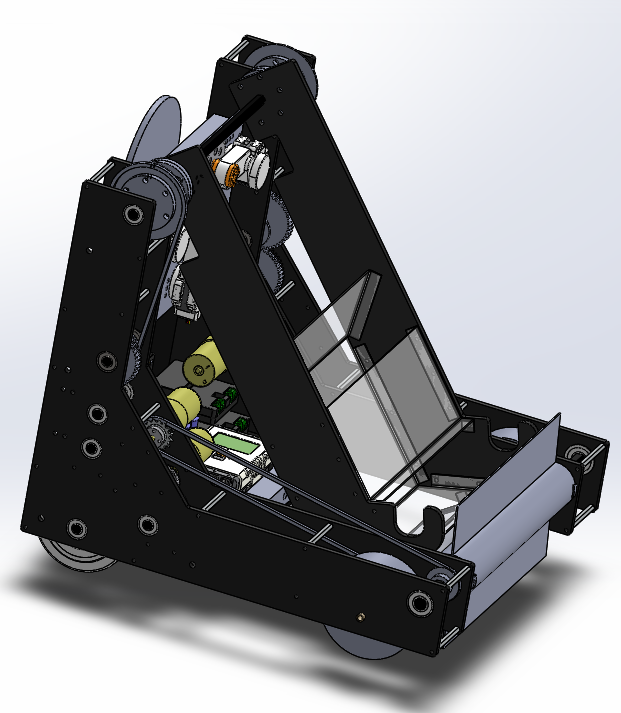
\includegraphics[scale=0.5]{images/RobotV1.png}
\end{center}
\caption{This is the first revision of our Solidworks. We can see the block acquisition device that is essentially a roller that will inhale blocks into our robot}
\end{figure}

Force is not an issue, and remains at a 16:1 ratio with torque gained. It is important to note that the force DOES double when an additional layer is added, however, with the 16:1 ratio between the movement of the bars, the speed with which the bars are raised ALSO doubles. This means that, though the force doubles, the speed at which the arm go up is also doubled. That implies that any torque issue created by adding another layer to the mechanism can be resolved by multiplying the gear ratio of the chain motor by two. The same vertical speed will be achieved.

The prototype is very functional. We connected it to the (makeshift) motor, and ran it. The mechanism lifted very well. The following problems were noted:
\begin{itemize}
\item Block pickup does not work
\item Lifting does not lock after power is lost
\item The wooden shaft collars strip
\item It does not move fast enough
\item It makes the robot very back heavy
\end{itemize}

Possible solutions to these problems (in order) are:
\begin{itemize}
\item Switch from the roller
\item Jam the gears
\item Change the wood to metal
\item Add steel to the front
\end{itemize}

Despite these issues, the lifting mechanism works well, and glides smoothly as long as they aren't stripped. Granted it is currently in prototype form, the final version (which will be produced much more carefully), should be very effective.

We are currently looking into redesigning the block pickup mechanism as it does not seem to be effective. We plan on lowering the roller to the ground and seeing what happens. 

Currently, our projected maximum height is 32”, just over what we need to hang on the bar.

\newpage \subsection{Flag Spinner Initial Test -- Meeting 6: 2013-10-6}
Today's meeting was short - it was only two hours. We had a couple ideas we wanted to test, and the tests were successful. We verified our idea would work, and redrew the pictures from two days ago.

The idea we were testing today was whether or not we could raise the flag by using a rubber-like substance to mesh within it and spin. We soon saw that the NXT motors were not as powerful as we would like and the force that the rubber plate was inducing was off center. This makes it unfeasible to use. 

\begin{figure}[H]
\begin{center}
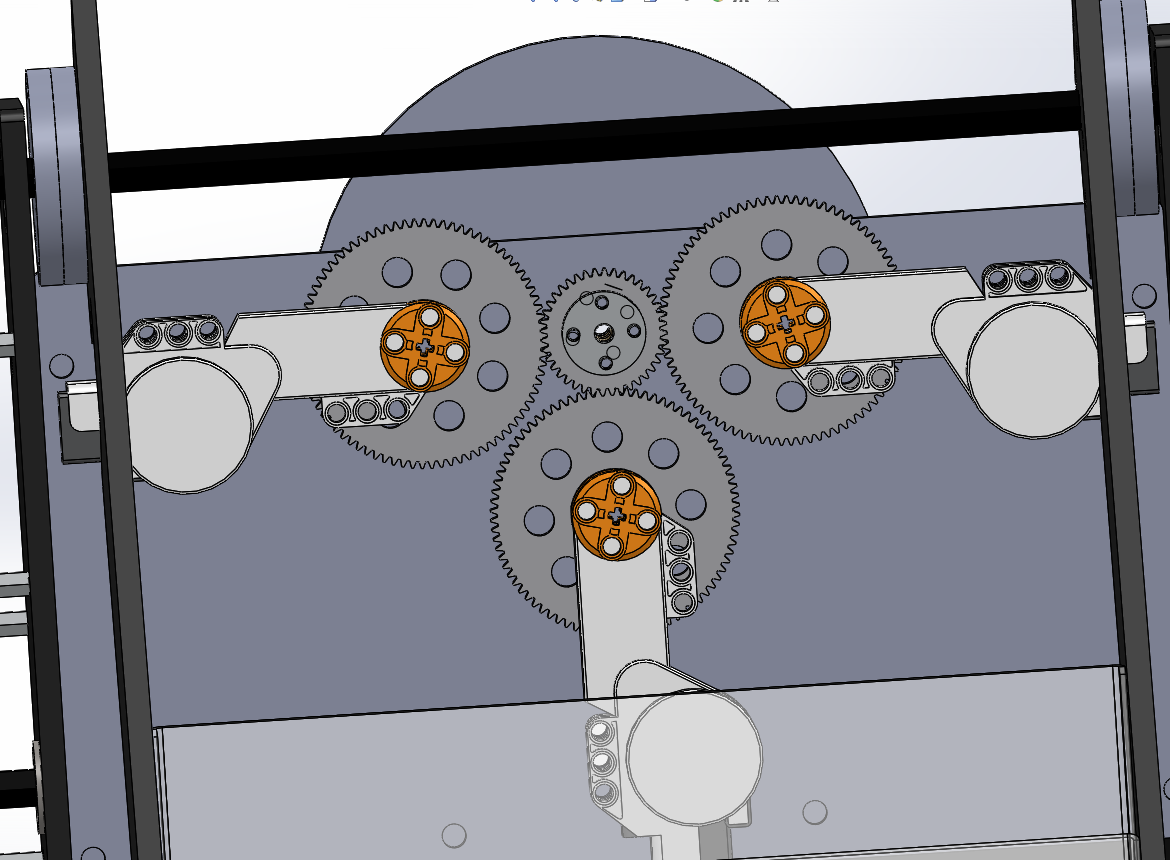
\includegraphics[scale=0.25]{images/FlagSpinnerV1.png}
\end{center}
\end{figure}


We plan on switching to the seemingly common extruded pins design. We plan on having two pins attached off center that are $180^\circ$ apart. We also plan on switching to a Tetrix motor with a $6:1$ gearing ratio. With this ratio, we will be able to raise the flag, theoretically, in under 10 seconds. 

However, this method adds an extra $1.5''$ to our length. As we must stay within the $18''$ length constraint, we may have to shorten our roller (block pickup mechanism). This may become problematic, but as far as we can see we should be able to work around it. 

For the pins, we had two ideas: the first is to use cut Tetrix axles. The second is to use longer Tetrix screws. We plan on using the Tetrix screws first to test and we may end up keeping them on afterwards. 

We also did some more testing with the roller. We experimented with lowering it and shrinking the radius of the aluminum tube. We chose a smaller inner radius due to the fact that it would weigh less and it would be easier to place near the ground. We are still running into issues of picking up much more than 4 blocks at a time. 

We decided on mounting it 1.5'' above the ground because this is just enough to let the blocks slide under as we roll. 

It is the popular idea that we want to completely redesign the block grabbing mechanism due to its inability to give us the accuracy and visibility that we want. Visibility is an issue when we go to the opposite side of the field. 

\newpage \subsection{Block Acquisition Redesign -- Meeting 7: 2013-10-11}
We have spent a lot of time working on scoring blocks, but we overlooked the difficulty of acquiring them. We decided to spend the day looking over our acquisition device as we found it was not very effective. We are looking into changing the roller into a much lower roller made of rubber. We are also looking into changing the entire design altogether. The main ideas revolve around driving into blocks and then flipping them into our arm. However, many members of the team do not like the idea of multiple moving parts. 

We decided to extend the final aspect of the roller and found that it was completely ineffective. There is currently no member that continuously supports this idea. 

Today, Garrison proposed that we use a bulldozer like system. A flat plate that we would use to ram into the blocks, which essentially extends our arm to be outside of the frame. We built a first prototype with this and it seems to show some promise. We are still unsure of the implications that this has for the a final working idea. It may also be easy for blocks to slip outside of our robot. 

We currently plan to go home and think about better ideas. We will probably have an in-depth Skype conversation over this idea. We look forward to improving this design as it needs a lot of work. 

The flag spinner was also entirely redesigned as follows:

\begin{figure}[H]
\begin{center}
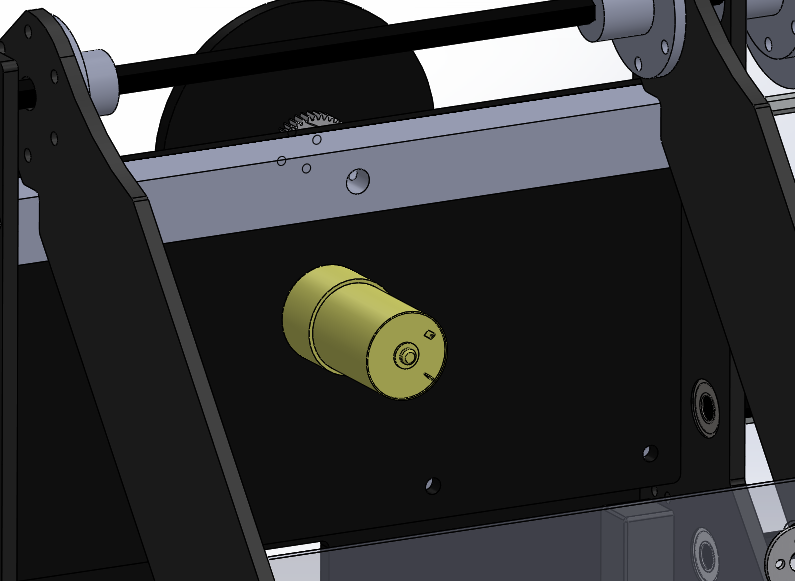
\includegraphics[scale=0.4]{images/FlagSpinnerV2Back.png}
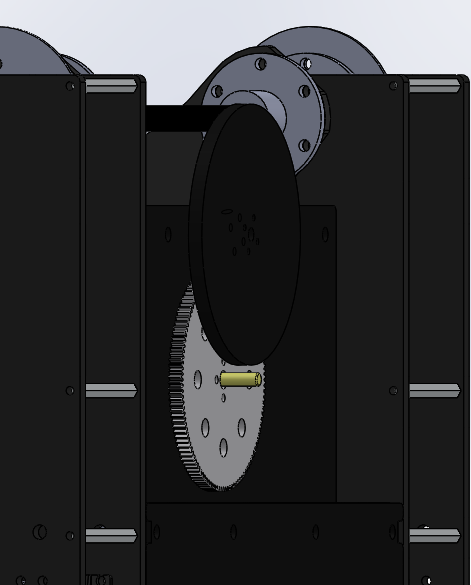
\includegraphics[scale=0.5]{images/FlagSpinnerV2Front.png}
\end{center}
\caption{Here we can see both sides of the new, redesigned, flag spinner. The notable changes include the switch to the Tetrix motor and the removal of the rubber backing in turn for extruding pins (not shown above).}
\end{figure}

\newpage \subsection{SolidWorks Redesign -- Meeting 8: 2013-10-18}
After coming back with new ideas, we spent the first hour of our meeting discussing the pros and cons of our new block acquisition mechanism. We all feel that a flat sheet on the ground that we can use to run into the blocks as a bulldozer is the optimal solution. 

We are designing it to be fully flush with the ground. We look forward to testing this out. In SolidWorks we are redesigning the base of the robot to be shorter to allow the bulldozer system to lie in front. 

\begin{figure}[h]
\begin{center}
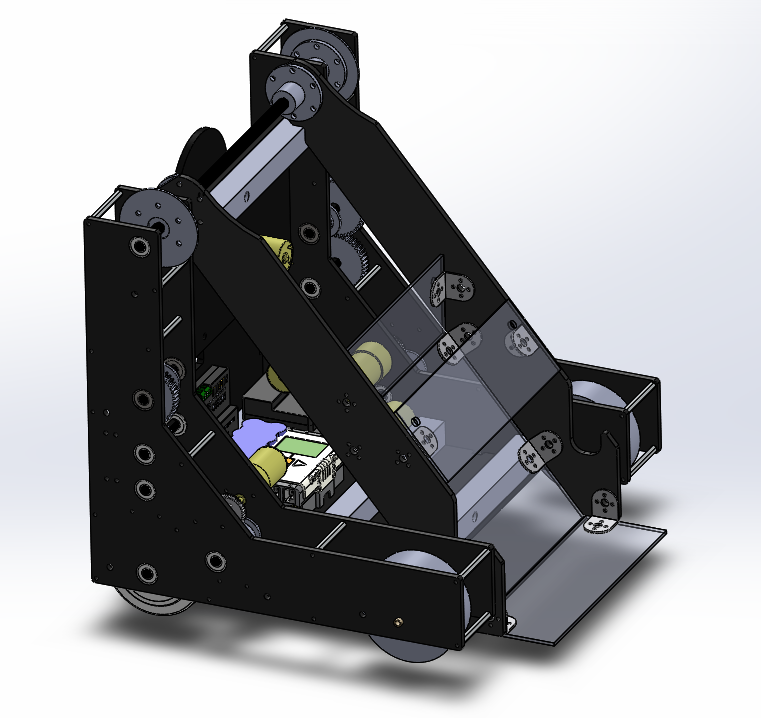
\includegraphics[scale=0.75]{images/RobotV2.png}
\end{center}
\caption{This is the second revision of our SolidWorks which includes the redesigned block acquisition device.}
\end{figure}

\newpage \subsection{First Full Test and Match -- Meeting 9: 2013-10-25}
Today was our first day with a complete robot. Although we had done several tests of our prototype before, this was the first day we had everything working together. The excitement within our team was immense. We tested our drive train with the added weight of the arm on the motor. We tied the flag mechanism with nylon as our Kevlar rope has not yet been received. The Kevlar provides less friction and is more like the competition.

Near the bottom, we have a lot of empty space to place the electronics. We hope to use the HiTechnic SuperPro this year to do much more sensor fusion. We want to add an Arduino or Atmel processor (ATUC3b0128) to do much more powerful computation without having to deal with the timing issues that are imposed by using the task system in RobotC and the slow clock of the NXT. We have plans to include gyroscopes, accelerometers and ultrasonic sensors. We are also looking into developing our own infrared seeker, although we are still uncertain about the feasibility of that task. 

With the A-frame design that we have we are able to distribute all of our weight to the back of the robot. This makes it very stable and very difficult to push us. 

When we scored our first block, the entire team was ecstatic. We all felt relief that we were able to lift something and score our blocks. We were somewhat surprised as to how simple it was for us to score a block - simply by driving backwards and raising the arm.

The arm went up very smoothly and we had no issues scoring on any of the blocks. We decided to play our first match to see how many points we were able to score.

We gave Tristan the controller and on our first run we were able to score about 200 points. We scored only on the outside baskets. This added up to the balanced bonus bonuses. Overall, we are very happy with the current design of the robot. Although, we do feel that a lot of driver practice is needed, along with an improved block acquisition device. 

Once we had the entire robot built we started testing the arm mechanism and its ability to remove and score blocks. We found that it requires almost no effort to manipulate, and that it has the force required to easily push under blocks.

Tristan, our driver, says that with the new ``fishtail'' drive train that we incorporated along with the ease of use of scoring blocks and removing them from the ground. We are still unable to consistently pickup four blocks. 

Now there is a lot of talk among the team members about autonomous and strategies for approaching the autonomous program. We have the ability to determine which column the Infrared beacon is one within one second of our robot starting up.

After we scored our first block and played our first game we decided that we had accomplished a decent amount for this extra Sunday meeting and decided to call it a day. We have high hopes for the competition and expect to place well at our first qualifier. 

\newpage \subsection{Short Design Meeting -- Meeting 10: 2013-11-2}
Today was mostly a day for driver practice and minor repairs. We did several hours of practice, then moved the grabbing mechanism down an inch because it was barely outside the sizing box. This created a couple functionality issues, which will be resolved in the next meeting. We also tested the autonomous accelerometer and gyroscope, but didn't get much farther than measuring the (mostly insignificant) error before we had to leave. 

Today was short.

\newpage \subsection{Tweaking and Autonomous Programming -- Meeting 11: 2013-11-8}
Today several mechanical changes were made. The flat block grabber was moved down more, but the attached aligning bars were kept in the same place. The bars were also melted into a curve to stop the blocks from catching on them, but at the same time keeping them from falling out. In addition, we made our hex arm shafts, designed after the AndyMark hex wheel shaft. We used a lathe to create the same shape and then used a hex broach of 3/8'' to allow it to slide over. 

Another notable change was somewhat small, but it was entirely necessary. We added a funnel system onto our arm to stop blocks from flying out as we tried to score. This was done with two small bent Tetrix pieces that redirect the blocks into the center of our scoring mechanism. 

After implementing this, the amount of blocks that we missed dropped from almost $50\%$ to nearly $2\%$. This worked phenomenally and outdid all of our expectations. 

Today was a rather complex code day. Yousuf and Kian woke up early to start work at 7 AM on autonomous. Other team members were arriving past 10. Our progress was significant and extensive, leading us into a few minor problems but also into several solutions. 

We decided immediately to write the code again from the bottom up, testing each component as we added it. The old code would have taken too long to get working properly. We struggled for around half an hour with a few simple glitches. We had a very silly error where RobotC simply refused to function properly. The eventual solution was ridiculous: the line of code with the error was replaced via copy and paste with a duplicate line from an old code file. This resolved the issue. 

Accelerometric integration now works, and we can properly integrate our position with very little noise and error. There are no issues here. 

The gyroscope integration, on the other hand, is returning garbage output. It's moderately representative of our actual rotation, but in actuality it is totally useless. The tolerance is +/- 10 degrees. I surmise this is a tasking issue, and $\delta t$ is not being set properly, resulting in error. 

We attached the infrared seeker sensors, and can now start the game consistently knowing which column the tag is in. We have a 540 degree field of view, since the two sensors face opposite directions. As such, our first movement command is to go directly to the column with the IR beacon. We may need to redesign our autonomous though since we are getting a lot of noise. 

Our plan is to turn perpendicular to the pendulum. Everything except the gyroscope is functional.

\newpage \subsection{Autonomous Working (No IR) -- Meeting 12: 2013-11-10}
This weekend, we successfully programmed our autonomous. The code allows the robot to deposit the autonomous block in any basket, as selected by the user interface. The logic for this decision works as follows:
\begin{itemize}
\item The user selects which row they would like the block placed in, if the IR beacon is in each column.
\item The robot uses triangulation with two outward-facing IR seekers to start the game immediately knowing which column contains the beacon. (This still doesn't work yet)
\item The robot angles to the correct basket.
\item The robot moves and rotates, aligning itself to score with the block.
\item The robot raises the arm, scoring the block.
\item It then backs off to move onto the ramp.
\end{itemize}

The program for this has been written, and works with an (approximated) 90\% consistency.

\newpage \subsection{Driver Practice and Lifting Locking -- Meeting 13: 2013-11-17}
The plan for the meeting was to spend an hour or two testing the autonomous for consistency at getting on top of the ramp. Then the plan was to do driver practice for the rest of the day.

Early tests of the autonomous showed some problems getting on top of the board, with the placement of the sensor being off about 30\% of the time. The most common issue occurred when the IR mounting was off center. This caused us major error. After mounting the beacon much more securely, the autonomous became very consistent at getting to the pendulum, scoring the vast majority of the time in several trials.

As we began driver practice, however, some structural problems were discovered. The cross bars that we were using to brace our lift torqued during one run, causing us concern when lifting. Tristan volunteered to create the crossbars in SolidWorks and spent some time taking careful measurements of the spacing between the two halves of the lift. The other major fix that was incorporated was to add two points of contact on each side in order to stop the arm from torquing under major force.

We also developed a lifting locking mechanism which works by jamming a third gear into our system. This induces a lock that cannot be broken and does not need power. Figure \ref{locking} shows this system in action.

\begin{figure}[H]
\begin{center}
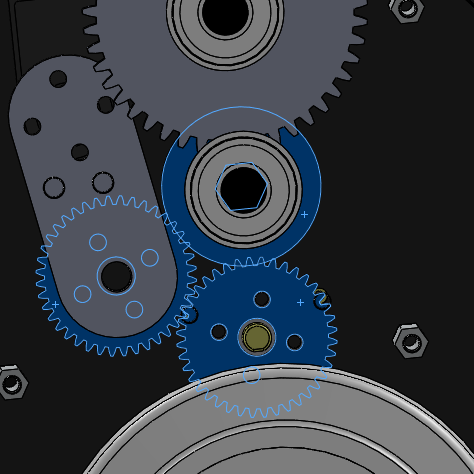
\includegraphics[scale=0.75]{images/Gearlock.png}
\end{center}
\caption{The blue sections highlighted show the three gears that are all locked together. It restricts any movement and works effectively.}
\label{locking}
\end{figure}

\newpage \subsection{Outreach -- Meeting 14: 2013-11-29}
This year we decided to mentor an FLL team and we mentored two FLL teams. We helped them program the new EV3 and taught them some new design techniques for the attachments that they had on their robot. We spent about 4 hours running through all of the programs they had and suggesting different ways that they could go about it. We also taught them how to use sensors as a lot of their programs were unreliable. We hope to start an FTC team with these students in the upcoming years. The FLL team we mentored just won their qualifier competition and has a regional competition at LegoLand on December 7th. 

\newpage \subsection{Driver Practice -- Meeting 15: 2013-12-6}
Today we mainly tested our robots abilities using time trials.  Our robot managed to pick up two to three blocks per trip, which was below our expectations.  Because of this we began experimenting with different methods of collecting blocks, such as a horizontal roller. The first material being a sheet of extremely thin sheet metal which was low enough to the ground but it was too weak, When we tried to pick up blocks the metal would buckle and make a wall impossible for anymore blocks to get up.  Our next solution was to use a thicker, flexible sheet of plastic that slid with really low friction across the ground.  The plastic sheet was just the right height to where it would fit perfectly under all of the blocks without getting deformed. 

Our next task was to be able to fit three or four blocks - no more, no less.  The way we solved this greatly important problem was by using a metal deterrent to block more than five blocks from being collected.  The combination of the ramp and the deterrent made it so that we extremely rarely picked up two blocks but we also very rarely picked up more than four blocks.

Overall, we are currently scoring approximately 300 points alone per round. We hope that our speed will be unmatched and we will be able to score many points. 
\newpage \subsection{After Competition Meeting and Revisions -- Meeting 16: 2014-01-06}
We took a break after the first competition to relax from robotics and think about how we did at our competition. We did very well being the winning team alliance and the Inspire Award Winners at the 2nd San Diego Qualifier. Once we met again we decided to fix the following issues: 

\begin{itemize}
\item Consistently pick up 4 blocks
\item Make raising our robot much quicker
\item Change the position of the autonomous block
\item Fix autonomous
\end{itemize}

We decided to work on moving the IR sensors to the side of the robot to make the control much more effective. To fix our consistency issues we widened the arm making it almost always pick up 4 blocks if we go on straight on. We also made it that we cannot pick up 5 or more blocks by adding an aluminum $\ell$ bar to prevent multiple rows of blocks.

We redid the logic of the autonomous program and it is now far more consistent.

\newpage \subsection{Pacific Ridge Qualifier Reflection}
The day didn't start off the best for our team. We started off the day with a scoop that wasn't exactly in the greatest condition, and our autonomous program wasn’t running optimally. By the time our first match came around, we started autonomous without a block scored, then were stuck on the walls and mangled two motors, leaving us with disabled robot. Needless to say, we lost that round. We needed to detach the side plates of our robot to remove and replace the two burnt motors. Thankfully, the kind teams we were competing with let us borrow motors. We have since given them replacement motors, and thanked them profusely for their generosity. 

Our next match went slightly better, but we managed to completely break our scoop. We could not fix it at the competition, as we had not brought spare plastic. Instead, we made an on the fly decision to cover our block scoop in duct tape. This temporary fix wasn’t very effective, but it worked, we won our next game but we were still in close to last. During our next game, we somehow managed to memory fault an NXT, destroying it completely. We were in around eight place during alliance selection. First picked second, then third picked us. In the elimination round of the qualifier we lost our first game but then won the next two. After that, we won our first game and lost our second, and when it finally came to our last match, we pulled the victory by quite a large gap.

We are looking to improve the consistency of our design so that similar errors do not occur in future competitions. The quantity of parts we had to borrow from other teams is simply inexcusable, and it was only the bounds of their generosity supporting our team. We are forever indebted to them, and will send back new parts posthaste.

\newpage \subsection{Glendale Qualifier Reflection}
We woke up at the crack of dawn the day of the competition. The robot had been moved to another team member’s house because Yousuf was out of town for an international science fair. We carpooled for the two hour drive up to the competition and stopped for some food. 

We were one of the first teams to arrive and quickly set up our pit for the competition. We had finished what we needed the day before, and were prepared for arrival. We passed inspection easily. However, our first game seemed to follow a familiar trend for destroying motors early in the competition. We successfully ran autonomous, but, one of our programmers left a piece of debug codethat caused the arm motors to burn out during teleop. As a result, we lost the two motors driving the arm. However, our mechanical problems stopped there. We remained undefeated for the rest competition. During alliance selection, we picked Syntax Error and The Millionaire Mind Kids for our partners. 

We remained undefeated for the rest of the elimination rounds and reached a personal high score with the Millionaire Mind Kids of 342 points. We also won the Inspire Award and qualified for the Los Angeles Regional Competition.

For futre competitions, we are looking to change the material of the platform used to pick up blocks, so that the mechanism becomes far more consistent and easier. We are also looking to widen the arm - while this could potentialy allow us to pick up five blocks, it is unlikely this will acutally happen in game. Hopefully, we will be able to pick up four blocks more consistently with these changes. We're looking forward to the regional competitions!   \newpage
\section{Software Architecture and Implementation}
Detailed in this section is the method and reason to our software architecture. In particular, we aimed for our architecture to be stateless with respect to the current operation, to maximize efficiency of joystick checks (which are normally slow in RobotC), and to allow dynamic and easy reassignment of both controller information during teleop, as well as both movement sequencing and heuristic decision trees during autonomous.

We have chosen a particular structure for our code. We have rewritten \lstinline{JoystickDriver.c}{} to better express our needs. By removing superfluous tasks from the driver, we maintained functionality while increasing our efficiency by approximately threefold. We have created a set of utility headers: \lstinline{teleoputils.h}{}, \lstinline{autoutils.h}{}, and \lstinline{sharedutils.h}{} to address the need for macros, \lstinline{#define}{} statements, and standardized functions. Both \lstinline{teleoputils.h}{} and \lstinline{autoutils.h}{} import \lstinline{sharedutils.h}{}, so that file is never explicitly included in the main code body. Drivers were pulled from HiTechnic's online library for 3rd party sensors.

\subsection{Teleoperated Mode}

Teleoperated mode has the following requirements: \begin{enumerate}
	\item{Smooth arcade driving}
	\item{Easy reassignment of buttons}
	\item{Stateless control of motors and robot state}
	\item{Efficient button control and loop checking}
	\item{\textbf{Must} use only one controller}
\end{enumerate}

In order to implement this effectively, we have implemented several macros. These macros allow us to later set the powers of the motors without much effort. 

\subsubsection{Drive Code and Reasoning}

Our main body of code is run through the following:

\begin{lstlisting}[tabsize=4]
task main() {
	while(true) {
		getJoystickSettings(joystick);
		checkJoystickButtons();
		setLeftMotors(powscl(JOY_Y1)-powscl(JOY_X1)/1.75);
		setRightMotors(powscl(JOY_Y1)+powscl(JOY_X1)/1.75);
	}
}
\end{lstlisting}

First, grab the current joystick configuration from the controllers. Then, check to see if any buttons have changed (\lstinline{checkJoystickButtons();}{}). Then, set the motor powers for arcade drive. 

\paragraph{Power scaling} The \lstinline{powscl(int)}{} function's definition is intended to compensate for the large deadband range which occurs under standard drive conditions. The controller's user really only needs two ranges: a high-precision, low power range near zero, and a low-precision, high power range near the maxima. While an exponential function could be used, it is much slower, and much more hard to tune. Instead, we draw two lines: a shallow slope for the first segment, then a large slope for the second segment of the controller. This provides both high precision and high power where needed. As the driver does not generally use the range in $[60,85]\%$, there is no concern about the nonlinearity. The function is defined as follows:

\begin{lstlisting}[tabsize=4]
float powscl(int xz) {
	float sign = (float)sgn(xz);
	float x = abs(xz)/128.0;
	if(x < DISTA)
		return 100* sign * (x*SLOPE);
	else
		return 100* sign * ((DISTA*SLOPE*(x-1.0) - x + DISTA) / (DISTA - 1.0));
}
\end{lstlisting}

\paragraph{Compensation for the Old and New Joystick Configuration} It is necessary to compensate for both the old and new controller configurations. As the controller has been updated, the buttons have changed - however, competition rules premit the use of both controllers. Therefore, we must be able to accomodate this change if necessary. We have done so through the use of a define statement: if we have \lstinline{#define ALTLOG}{}, then we switch to the old button layout.

\paragraph{Button Press Checking Requires a Stateless Organization} In order to easily and effectively change the functionality of the controller, a particular design was implemented:

\begin{lstlisting}[tabsize=4]
void invokeButton(int button, bool pressed) {
	switch(button) {
		case JOY_X:  if(pressed) {servo[servoL1] = 156; servo[servoL2] = 26;} else {} break;
		case JOY_Y:  if(pressed) {servo[servoL1] = 120; servo[servoL2] = 40;} else {} break;
		case JOY_A:  if(pressed) {} else {} break;
		case JOY_B:  if(pressed) {motor[mSpin] = 100;} else {motor[mSpin] = 0;} break;
		case JOY_RB: if(pressed) {setArmMotors(100);}  else {setArmMotors(0);} break;
		case JOY_LB: if(pressed) {setArmMotors(-100);} else {setArmMotors(0);} break;
		case JOY_R3: if(pressed) {} else {} break;
		case JOY_L3: if(pressed) {} else {} break;
	}
}

bool t[8];
void checkJoystickButtons() {
	for(int i = 0; i < 8; i++) {
		if(joy1Btn(i) != t[i]) {
			invokeButton(i, !t[i]);
			t[i] = !t[i]; 
		}
	}
}
\end{lstlisting}

This may appear confusing at first, however, there are a couple points: \lstinline{checkJoystickButtons()}{} is actually called from the main loop. It simply checks to see what buttons have changed on the controller, and calls the appropriate \lstinline{invokeButton(int, bool)}{} arguments. In doing so, we can determine exact behavior on button presses with ease. As our robot is very simple, we do not need more than a handful of buttons, so most of them remain unassigned.

\newpage \paragraph{Code Optimizations} Although this method works for determining which button is being pressed, we quickly found it is not the most elegant way of doing so. First off, we use a \lstinline{bool[]}{} to hold the state of each button. This seems intuitive, but the RobotC compiler actually creates an entire \lstinline{char}{} to hold either \lstinline{true}{} or \lstinline{false}{} for every \lstinline{bool}{}; this is a waste of memory. The other issue can be found in the processing structure. Each iteration of the program checks all possible button conditions; this is a waste of processing time if there has been no change since the last iteration.

\begin{lstlisting}[tabsize=4]
short btn = JOY_BTN;//local store = live store, initially
void checkJoystickButtons() {
	if(btn == JOY_BTN) return;//checksum
	for(short i = 11; i >= 0; i--) {
		if((btn>>i) ^ (JOY_BTN>>i)) {//check each button for a change
			invokeButton(i, ((btn & (1 << i)) == 0));//trigger event (#, down|up)
			btn ^= 1<<i;//mirror changes in local store
		}
	}
}
\end{lstlisting}

We solve the former issue by means of storing each button state in a single bit of data, reducing our memory footprint. Teams are encouraged to call the \lstinline{joy1Btn(int)}{} function each time they wish to check the state of a particular button, but this can become cumbersome of one wishes check multiple buttons in real-time. The ``JoystickDriver.c'' file that we must use for field communications stores each button state in a single \lstinline{short}{}; this means that we are capable of running a checksum of the joystick state before we check each button. This not only reduces our time per iteration, but also allows for our robot to be more responsive to joystick changes due to the inherent speed of bitwise operations.

\newpage \subsection{Autonomous Mode}
Autonomous, much like teleop, must meet certain criteria: \begin{enumerate}
	\item{Recognize which crate has been chosen with the IR beacon}
	\item{Move to said crate in a timely manor}
	\item{Move to onto the bridge after scoring our block}
	\item{Avoid any other robots on the way}
\end{enumerate}

\paragraph{Crate Detection} Much like any other team, we use the HiTechnic IR Seeker to determine which crate our robot should pursue. We use a function that reads not only the position of the IR beacon relative to our location on the field, but also the strength at which it is reading. Having more than one variable to check greatly reduces the generally unavoidable environment-error the comes hand-in-hand with Infrared Light detection.

\paragraph{Movement Functions} Using motor encoders, sensing how far a robot has moved is relatively simple in theory. Generally, the code becomes messy when the programmer has to remember motor encoder values and direction. To solve this issue, we have implemented general movement functions based on inches.
\begin{lstlisting}[tabsize=4]
void rbtMoveFdTime(float inches, int msec) {
	int enc = getEncoderByInches(inches); clearEncoders();
	int norm = -1.0*sgn(inches);
	ClearTimer(DrTimer);
	while(leftEncoder < enc && rightEncoder < enc && time1[DrTimer] < msec) {
		setLeftMotors (100*norm);
		setRightMotors(100*norm);
	}
	setLeftMotors(0); setRightMotors(0);
}
\end{lstlisting}
This function allows our robot to move forward by a arbitrary number if inches and finish the motion in less than the specified time. Generally one does not want to move forward for an amount of time because the power fluctuates with battery levels. On the same hand, if one moves forwards based on just encoder values, the motor have the potential to burn out if the robot incurs a collision. Allowing the function to reach the specified distance before a certain amount of time insures that neither of these situations have a high probability of surfacing.

\paragraph{Object Avoidance} Through the use of the HiTechnic SuperPro that was made legal by this year's game manual, we have been able to mount a high performance ultrasonic sensor to validate that the path we wish to take is open. If there is an obstruction, the robot moves onto the bridge via an alternate route. This feature increases the probability of a higher average score.

\begin{lstlisting}[tabsize=4]
bool pathClear(float dist){
	pause();
	float read = 0;
	for(int i=0;i<10;i++){read+=(analogRead(A3)*0.4);wait1Msec(5);}
	nxtDisplayBigTextLine(3,"%f", read/10.0);
	wait1Msec(2000);
	return ((read/10)<dist?false:true);
}
\end{lstlisting}

\newpage \subsection{Algorithms and Cartesian Mathematics}

\subsubsection{Hybrid Localization Using Gyroscopes \& Odometers}
\paragraph{Odometric Data}
We begin by assigning the following constants: 
\[D_{ot}=\frac{\text{Distance}}{\text{odometer tick}}=\pi(\text{wheel diameter})/(\text{ticks/revolution})\]\[ \theta_{ot} = \frac{\theta}{\text{odometer tick}} = \pi\left(\frac{\text{wheel diameter}}{\text{distance between wheels}}\right)/(\text{ticks/revolution})\]
We can calculate $(x_{\mathrm{enc}}, y_{\mathrm{enc}}, \theta_{\mathrm{enc}})$ from the odometer as follows: 
\begin{center}
	\begin{align*}
		\mathrm{d}l &= l^t_{\mathrm{enc}}-l^{t-1}_{\mathrm{enc}} \\
		\mathrm{d}r &= r^t_{\mathrm{enc}}-r^{t-1}_{\mathrm{enc}} \\
		\mathrm{d}D &= \frac{1}{2}(\mathrm{d}l+\mathrm{d}r)D_{ot} \\
		\mathrm{d}x_{\mathrm{enc}} &= \mathrm{d}D\cos(\theta^t_{enc}) \\
		\mathrm{d}y_{\mathrm{enc}} &= \mathrm{d}D\sin(\theta^t_{enc}) \\
		\mathrm{d}\theta_{\mathrm{enc}} &= (\mathrm{d}r-\mathrm{d}l)\theta_{ot} \\
		x_{\mathrm{enc}} &= x^{t-1}_{\mathrm{enc}} + \mathrm{d}x_{\mathrm{enc}} \\
		y_{\mathrm{enc}} &= y^{t-1}_{\mathrm{enc}} + \mathrm{d}y{\mathrm{enc}} \\
		\theta_{\mathrm{enc}} &= \theta^{t-1}_{\mathrm{enc}} + \mathrm{d}\theta_{\mathrm{enc}}
	\end{align*}
\end{center}

$l$ denotes the left side of the robot, and $r$ denotes the right side of the robot. $D$ denotes the distance. 

\paragraph{Localization Algorithm}
The robots motor controller calculates position and orientation $(x_{\mathrm{enc}}, y_{\mathrm{enc}}, \theta_{\mathrm{enc}})$ from encoder ticks and sends the data to an on-board computer. The mounted gyroscope communicates with a gyro driver which integrates the rate values into an absolute angle ($\theta_{\mathrm{gyro}}$). Global position $(x_{\mathrm{rbt}}, y_{\mathrm{rbt}})$ is found by transforming the translation vector from encoder space to gyroscope space. Global angle $(\theta_{\mathrm{rbt}})$ is the gyro angle ($\theta_{\mathrm{gyro}}$). The following describes the computation as an iterative algorithm: 

\begin{center}
	\begin{align*}
		\mathrm{d}x&=x^{t}_{\mathrm{enc}}-x^{t-1}_{\mathrm{enc}} \\
		\mathrm{d}y&=y^{t}_{\mathrm{enc}}-y^{t-1}_{\mathrm{enc}} \\
		\mathrm{d}\theta&=\theta^t_{\mathrm{gyro}}-\theta^{t}_{\mathrm{enc}} \\
		x^t_{\mathrm{rbt}}&=x^{t-1}_{\mathrm{rbt}}+\cos(\mathrm{d}\theta)\mathrm{d}x-\sin(\mathrm{d}\theta)\mathrm{d}y \\
		y^t_{\mathrm{rbt}}&=y^{t-1}_{\mathrm{rbt}}+\sin(\mathrm{d}\theta)\mathrm{d}x+\cos(\mathrm{d}\theta)\mathrm{d}y \\
		\theta^t_{\mathrm{rbt}}&=\theta^t_{\mathrm{gyro}}
	\end{align*}
\end{center}
       \newpage
\section{Outreach}
As a team, de.evolution believes that robotics is more than just the engineering. Our first year as a team we saw that the other FTC team at our school, Domo Arigato, was entirely seniors and we were sad that it was going to disappear. This inspired us to try and spread robotics to the younger students and have people involved to keep robotics teams going and to propogate the message of FIRST throughout our community. We have started a robotics class at our high school which has turned into the team Domo Arigato. Due to the popularity of the class a second class, and subsequently an FTC team, has been started. Both the Robo Ravens and Domo Arigato, along with our own team, de.evolution, work hard to start a robotics and engineering culture at our school. The section will be structured as follows, we will begin by listing our community outreach and will in the subsequent subsections go into further detail about some of the more important work we do

\subsection{Community Outreach}
As a team, de.evolution has tried to do a lot to help spread the ideas of FIRST, robotics and engineering. The following is an extensive list of some of the community outreach that we have done:

\begin{enumerate}
\item Robotics demos to elementary school students at Solana Pacific Elementary, Del Mar Heights Elementary, Rancho Santa Fe Elementary
\item PTC World demo in June 2013
\item Mentoring of the three Islamic School of San Diego FLL teams 
\item Sister team of the San Dieguito Academy FTC teams Paradox Squared and Paradox Cubed
\item Demo for school board \& superintendent – sponsored building/engineering production district-wide with bond measure
\item Hosted Robotics Week at CCA in coordination with Domo Arigato
\item Publication in newspapers \& press releases about stem/robotics
\item Publication in school's magazines
\item Over 20\% of school has become involved with the FIRST robotics programs after the inception of our team
\item Inspired the FIRST robotics classes
\item Incorporating art and conservatory at CCA with the robotics program
\item Incorporating the humanities conservatory at CCA with the robotics teams
\item Working with TEDxYouth@SanDiego to spread robotics to the students in San Diego
\item Hosted small scrimmages at home
\item Hosting fundraisers at Souplantation for FIRST robotics
\item Attended and presented at Rotary meetings to show our community the influence of robotics
\end{enumerate}

\subsection{Helping other teams online}
As the majority of the members on our team are also on the FRC team \underline{The Aluminum Narwhals} we realize that having online support is one of the best ways to debug and learn about robotics. Chief Delphi, one of the prominent places for online FIRST discussion, is very popular among FRC teams. However, FTC teams do not have nearly as much online support as they may need or like. As a team we have shifted a lot of our focus to helping teams online. We have open-sourced all of our code and have created code tutorials to help out many other teams. In specific we have helped teams in the following ways:

\subsubsection{Syntax Error code optimization assistance}

At a San Diego regional qualification competition, we entered a discussion with team 6077, Syntax Error, about code optimization. We were sharing our varied tricks which were used in code, and through discussion, it became clear that there were a couple points they were particularly interested in implementing. We passed them some contact information, and later received an email from them:

\begin{lstlisting}
Hey Noah,

We're interested in optimizing the speed of our teleop code, and I know you had mentioned at the tournament that you guys XOR-ed the joystick values to determine when the values had changed--allowing you to skip checks when things weren't changing. Could you please go into more depth as to how you achieved this? Did you directly modify joystickdriver.c? Which values should we be XOR-ing exactly?

Thanks,
-Collin 
\end{lstlisting}

We wrote out a document generally detailing the approaches we took when optimizing our teleoperated code. My response was the following PDF file:

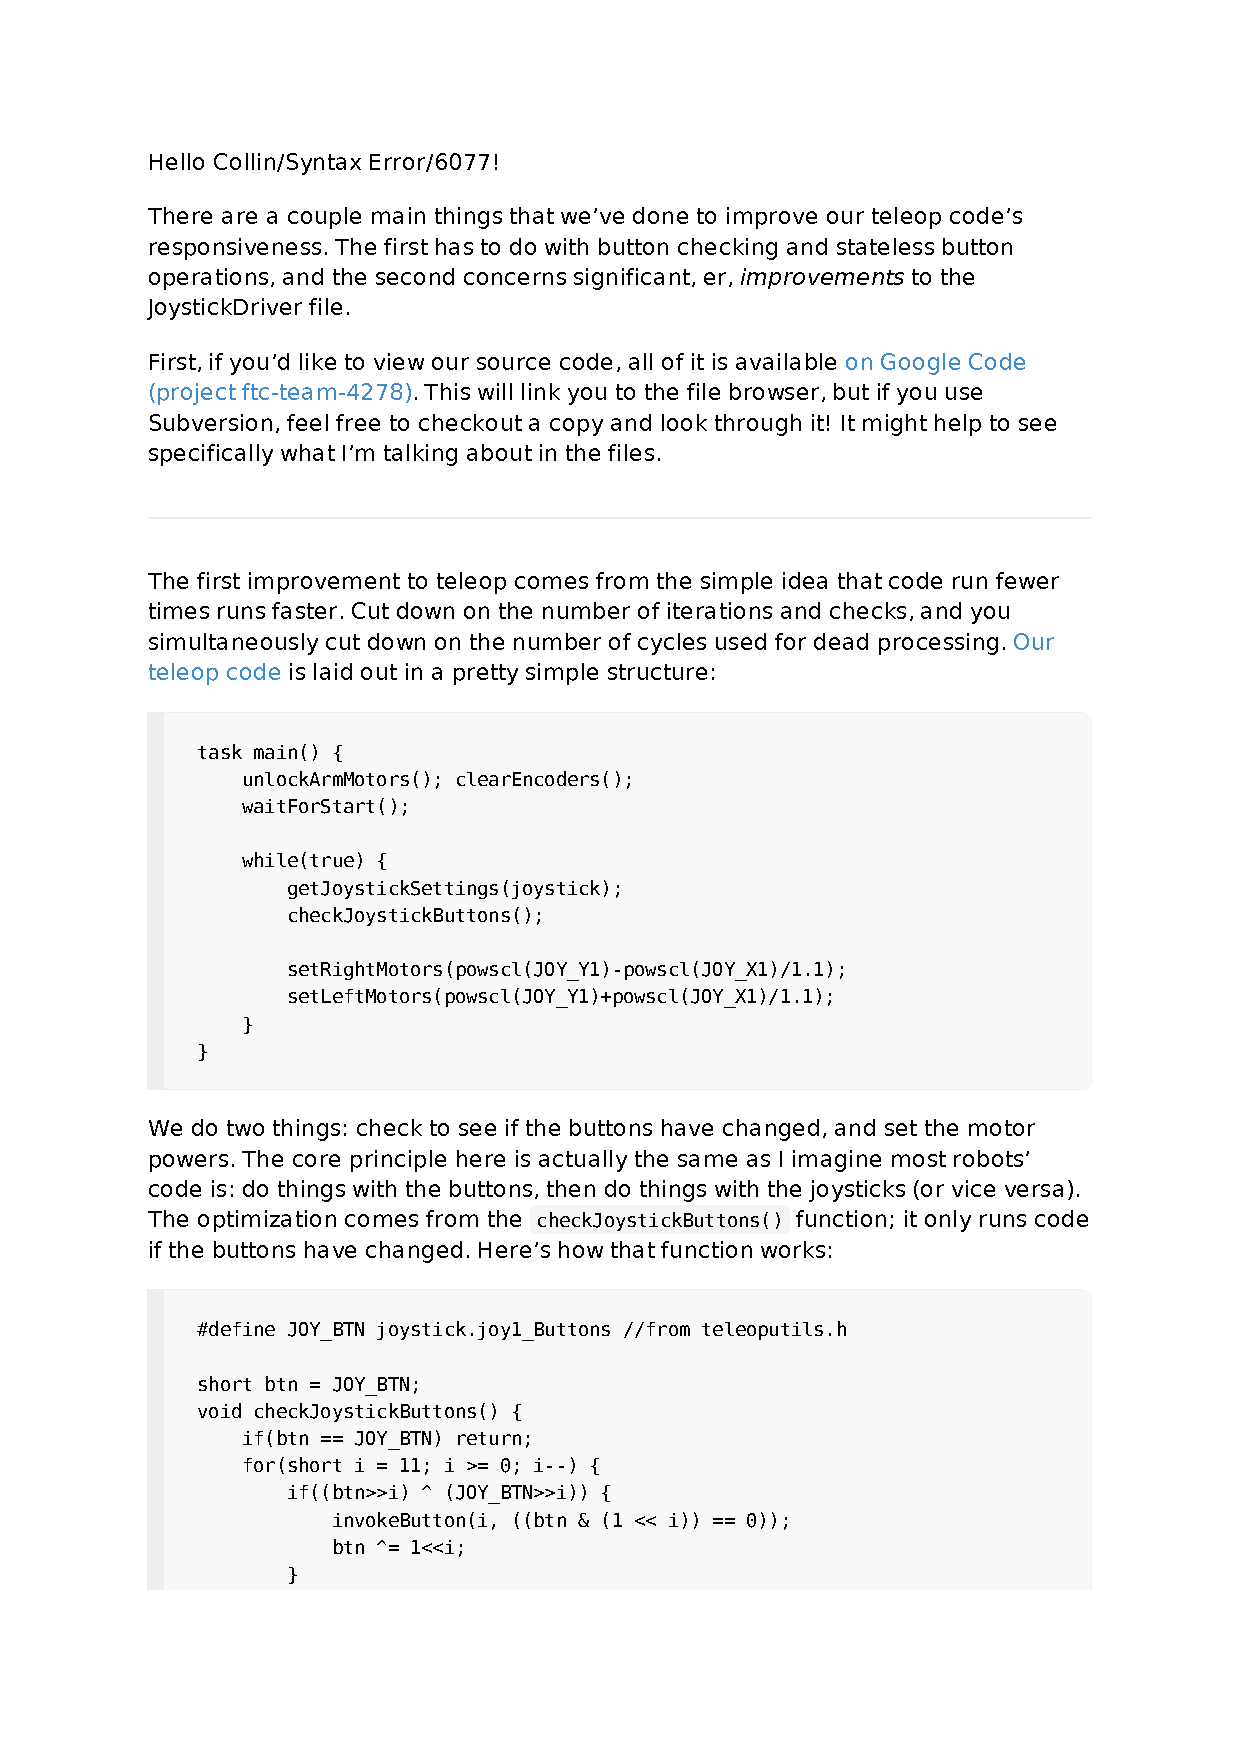
\includepdf[pages={1-2}]{SyntaxError.pdf}

The aim was to create an easy-to-follow guide for someone with experience to optimize the teleoperated program. To our enjoyment, they reported significant increases in response time on their controller.

\subsubsection{Reddit}

\subsection{Mentoring of FLL teams}
Our team aided the Islamic School of San Diego's FLL Teams during their rookie years by mentoring the young kids on robotics and the engineering design process in general. Our students voluntarily watched over the excited and energetic children, assisted in teaching them key concepts, and created useful PowerPoint presentations that were presented to further educate the FLL teams.

In each meeting, the FLL teams was taught a concept and then given time to build something from LEGOs using their newfound knowledge. Since our de.evolution volunteers were there, the FLL leader could split the team into small groups with a mentor or leader helping each group. Another advantage of having an FTC mentor available was that the volunteer could lead the team while the leader temporarily prepared the next lesson or dealt with other essential tasks. It relieved the leader of FLL and kept everything running smoothly.

The lessons taught the eager and energetic students about what causes earthquakes and the destruction that they inflict. This understanding supported the kids in cooperatively creating ideas for a machine to aid anyone who recently experienced a devastating disaster. The mentors also educated the group about the engineering design process to assist them in efficiently building a better solution when they were ready to begin fabrication of their product.

We found that mentoring FLL teams has not only allowed us to teach the students a lot about robotics, but we gained valuable experiences by doing so.
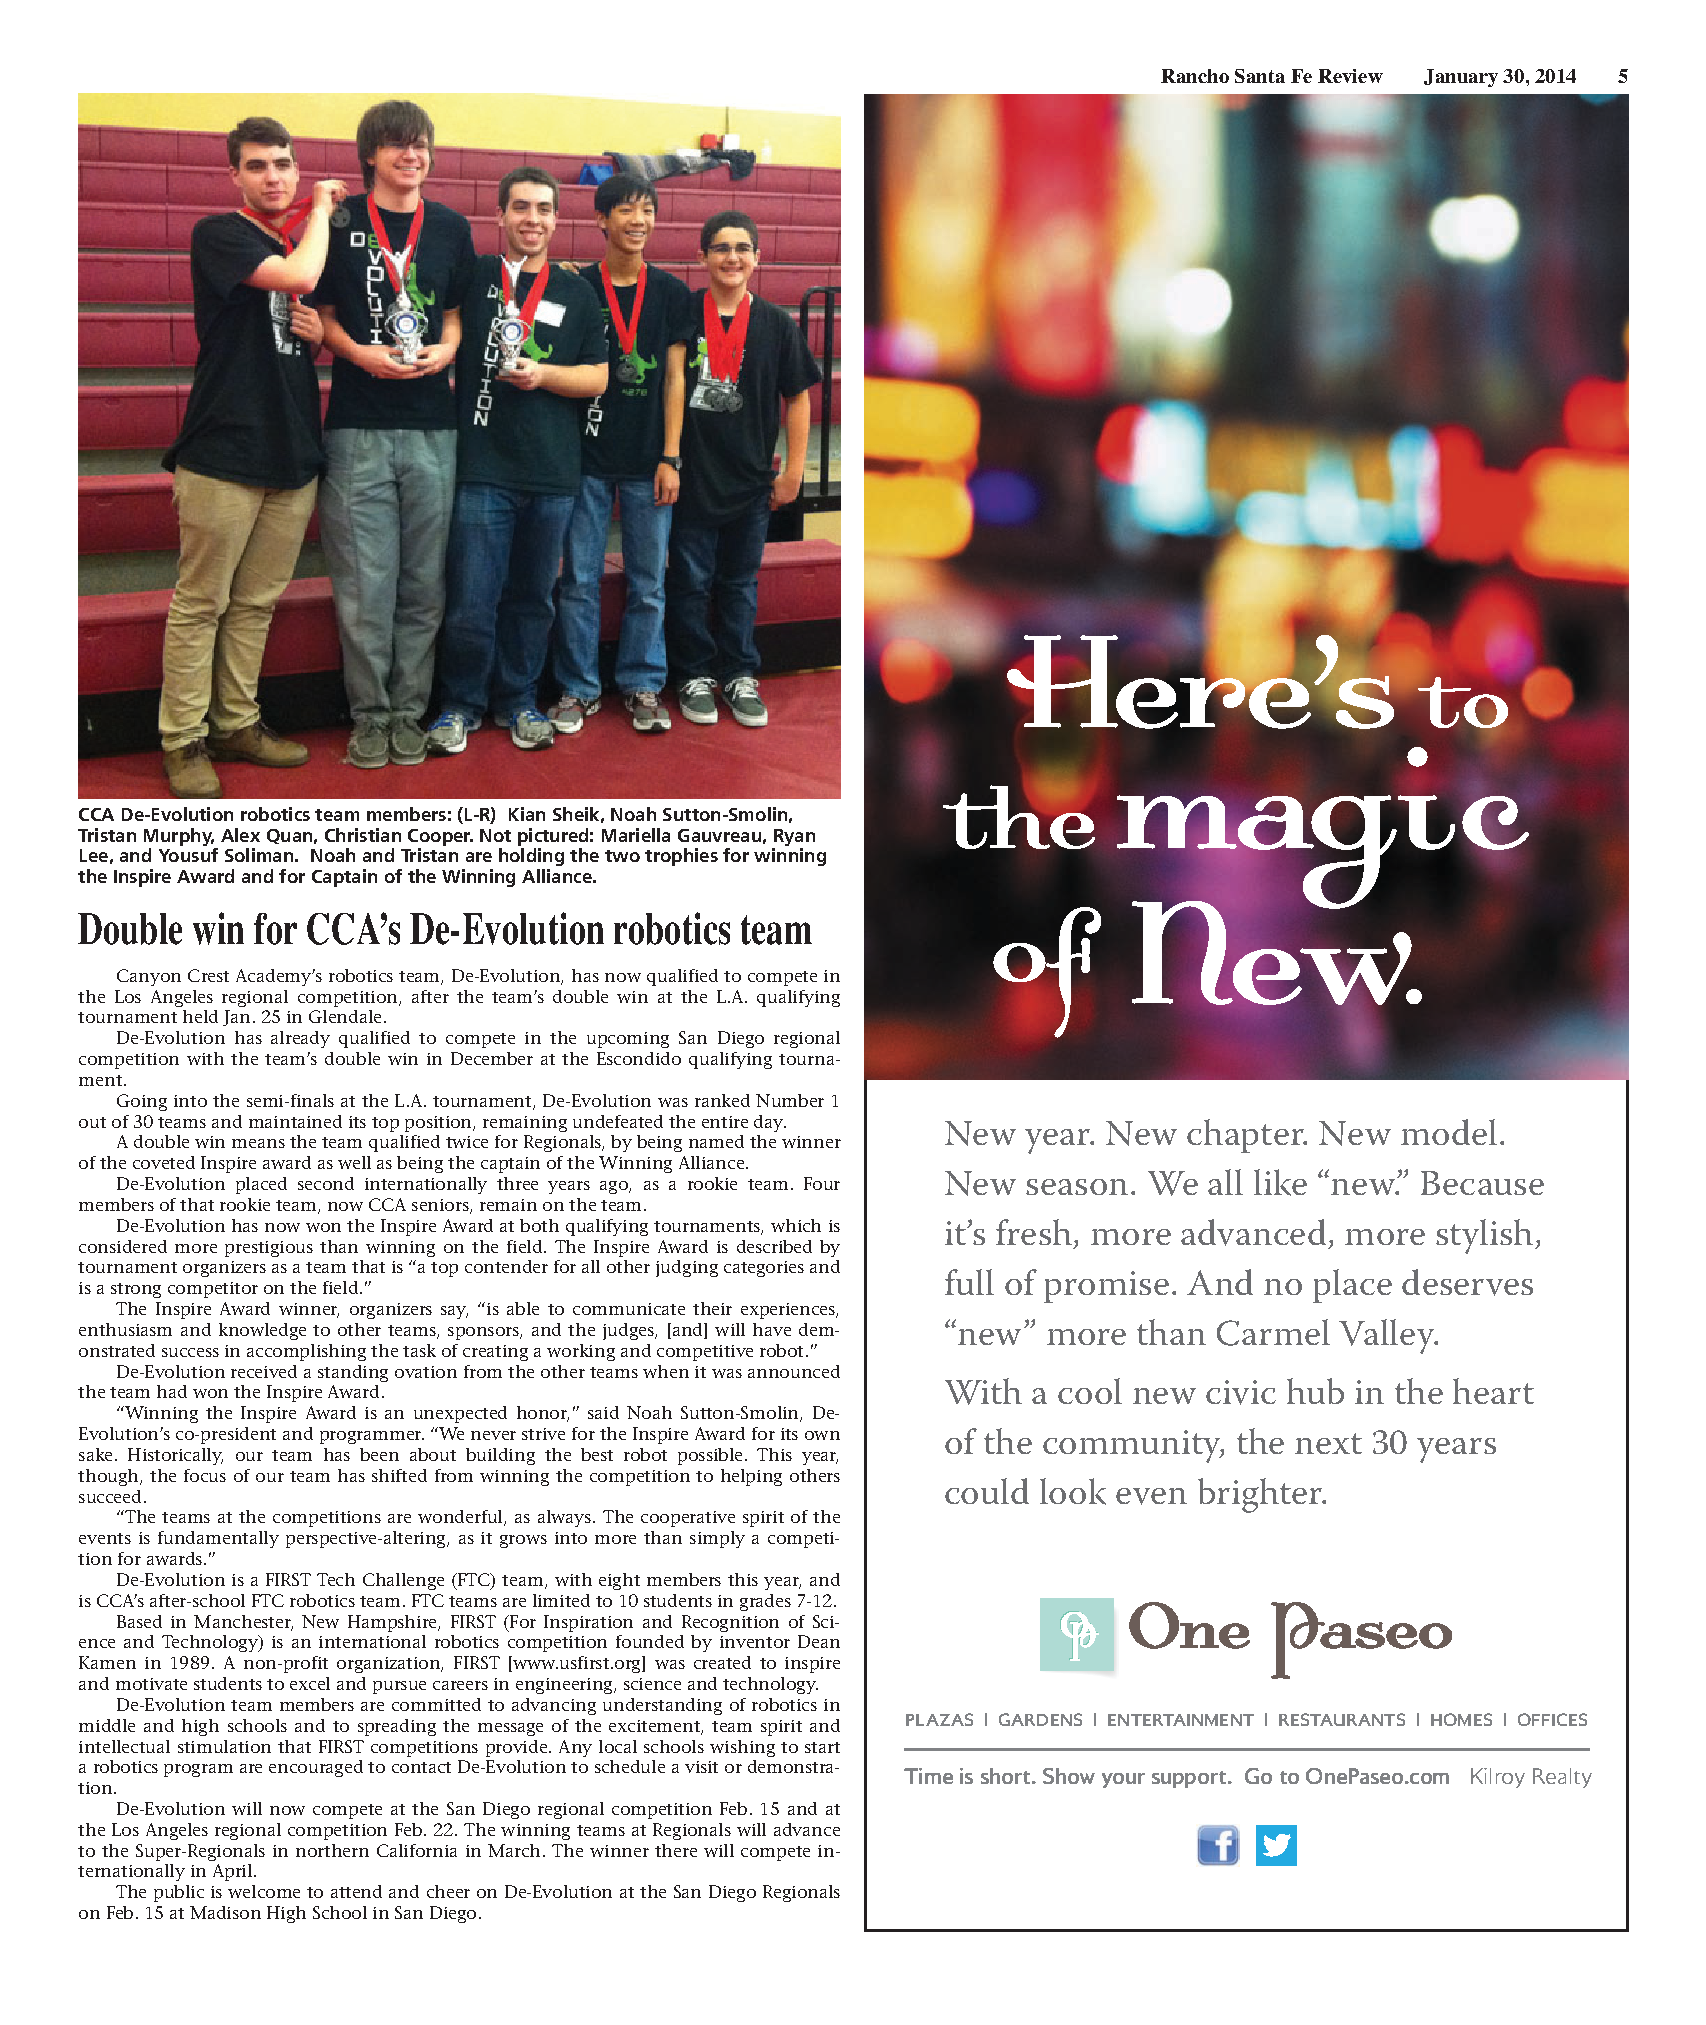
\includepdf[pages={-}]{DoubleWinNewspaper.pdf}

   \newpage
\section{Team scoring and ranking application}

It is difficult to deny a certain degree of randomness in the FTC competitions. While the competitions are fair and the sample size is large, the ranking points and qualifying points do not necessarily give a clear picture as to the difficulty of the competition or the overall effectiveness of a specific team.

In order to mitigate this problem, we have created our own method for ranking teams fairly based on how well they perform in each match. This allows us to provide a cleaner and easier ranking system for teams, which gives them due credit for the quality of their robot and design.

Let us assume, for instance, that two very good teams are up against one very good team and a moderately good team. Statistically speaking, it is more likely for the two very good teams to win the match. The current ranking point system accomodates this by only giving the winning teams ranking points. While this is, for the most part, fair and effective, there are certain cases under which teams are not necessarily given equal competition - or, even, that a team was lucky in their match selection. 

With our scoring and ranking app, we mitigate this problem in a few critical ways. While the FTC competition's scoring measurements are fair and accurate, the program we designed gives better insight into how much specific teams are actually helping their alliance partners, and allows teams to make more clear decisions about who they may wish to pick during alliance selection. 

The algorithm is composed of three steps:

\begin{enumerate}
\item The algorithm finds the average match score for each team
\item The algorithm then finds how much that average score was changed by a specific alliance
\item The algorithm then adds those together to produce a final score - the ``power rank'' for each team
\end{enumerate}

These three steps combined do several unique things. However, the most important of these is that \textbf{the algorithm gives teams credit for how much they assist their alliance's overall score.} This means that if you help your alliance - even if you don't win the match - you're still credited for your assistance in that match. 

In this way, it becomes irrelevant how well the players do in ther competition; rather, it simply becomes relevant how well the individual team does when contributing to their alliance score. This is the ultimate goal of the algorithm: instead of measuring the competition, measure the individual robot.

Over the course of the program's use and execution, we have noted several distinct cases where teams who are, in all honesty, quite good, do not end up as a match seed or even necessarily near the top - instead, they have lost many of their matches. It becomes clear when looking at match records that such teams are often pitted against the hardest teams to beat, and so the ranking points may not necessarily be the best representation of their success as an FTC team.

We do appreciate FIRST's method for ranking teams at the competiton, however. It's very straightforward, clear-cut, and promotes healthy and friendly competition. The method we use, however, is designed more so for fairness to the individual teams than it is for the actual rankings themselves.

\textbf{We make the results of these analyses public.} At each competition, we have had multiple teams ask to see our ranking results, simply because they would like to know where their team lies, or because they would like to gather a clearer picture of which teams may be better to pick. Either way, it would be unfair of us to keep these results to ourselves, so we make them available for broader use. \newpage
\section{Code Appendices}
The following code appendices detail our code, and a very high-level explanation of the code's intent and architecture.

Additionally, all of our code is available on Google Code.

\subsection{Teleoperated code}
\begin{lstlisting}
#include "drivers/teleoputils.h"

void invokeButton(int button, bool pressed) {
	switch(button) {
		case JOY_X:  if(pressed) {setSpinMotor(100);}  else {setSpinMotor(0);} break;
		case JOY_Y:  if(pressed) {setSpinMotor(100);}  else {setSpinMotor(0);} break;
		case JOY_A:  if(pressed) {setSpinMotor(100);}  else {setSpinMotor(0);} break;
		case JOY_B:  if(pressed) {setSpinMotor(100);}  else {setSpinMotor(0);} break;

		case JOY_RB: if(pressed) {setArmMotors(50);}  else {setArmMotors(0);} break;
		case JOY_LB: if(pressed) {setArmMotors(-100);} else {setArmMotors(0);} break;
		case JOY_RT: if(pressed) {unlockArmMotors();} else {} break;
		case JOY_LT: if(pressed) {lockArmMotors();} else {} break;

		case JOY_R3: if(pressed) {} else {} break;
		case JOY_L3: if(pressed) {} else {} break;
		case JOY_ST: if(pressed) {} else {} break;
		case JOY_BA: if(pressed) {} else {} break;
	}
}

short btn = JOY_BTN;
void checkJoystickButtons() {
	if(btn == JOY_BTN) return;
	for(short i = 11; i >= 0; i--) {
		if((btn>>i) ^ (JOY_BTN>>i)) {
			invokeButton(i, ((btn & (1 << i)) == 0));
			btn ^= 1<<i;
		}
	}
}

void debugBlock() {
	nxtDisplayTextLine(0,"%d",rightEncoder);
	nxtDisplayTextLine(4,"%d",joystick.joy1_TopHat);
	int dirIR, strIR;
	HTIRS2readEnhanced(sensorIR, dirIR, strIR);
	nxtDisplayTextLine(1,"IR: %i", dirIR);
	if(dirIR == 5) {
		PlaySound(soundBeepBeep);
		setRightMotors(0); setLeftMotors(0);
		setArmMotors(0);
		while(1 == 1) wait1Msec(5);
	}
}

task main() {
	unlockArmMotors();
	clearEncoders();
 	waitForStart();

 	while(true) {
		getJoystickSettings(joystick);
		checkJoystickButtons();
		//debugBlock();

		setRightMotors((powscl(JOY_Y1)-powscl(JOY_X1)/1.1));
		setLeftMotors(0.8*(powscl(JOY_Y1)+powscl(JOY_X1)/1.1));
	}
}
\end{lstlisting}

In essence, our code has two sections: check to see if the buttons have changed, and set the power of the drive motors. This has the effect of keeping the speed of execution high - it doesn't run the button code every iteration, but only if the buttons have actually changed.

\subsection{Autonomous}
\begin{lstlisting}
#include "autoconst.h"
#include "drivers/autoutils.h"
//#include "drivers/autodummy.h"

int OPT_SIDE = 0; int OPT_AUTO = 0; int OPT_DELAY = 0; int OPT_BRIDGE = 0;

void initializeRobot() {unlockArmMotors();}
void moveToBridge() {
	setLeftMotors(60*LEFT_POW_DIFF);
	setRightMotors(60*RIGHT_POW_DIFF);
	wait1Msec(3000);
	setLeftMotors(0);
	setRightMotors(0);
}

void runAutoLeft() {
	int irEncDist = -1;
	     if(OPT_AUTO == 0) {irEncDist = rbtMoveToIR(C4_ENC, 6000) - getEncoderByInches(IR_REALIGN); rbtMoveFdEnc(IR_REALIGN, 2000);}
	else if(OPT_AUTO == 1) {rbtMoveFdEnc(C1_ENC, 5000); irEncDist = C1_ENC;}
	else if(OPT_AUTO == 2) {rbtMoveFdEnc(C2_ENC, 5000); irEncDist = C2_ENC;}
	else if(OPT_AUTO == 3) {rbtMoveFdEnc(C3_ENC, 5000); irEncDist = C3_ENC;}
	else if(OPT_AUTO == 4) {rbtMoveFdEnc(C4_ENC, 5000); irEncDist = C4_ENC;}

	rbtArcRight(90);         //Turn to crate
	rbtMoveFdDist(4, 3000); //Against crate
	dumpArm();               //Dump blocks
	rbtMoveFdDist(-1, 1000);  //Back away

	if(OPT_BRIDGE == 0) OPT_BRIDGE = C23_THRESH < irEncDist ? 2 : 1;
	if(OPT_BRIDGE == 1) { //Left
		rbtArcLeft(90);
		rbtMoveFdEnc(irEncDist+getEncoderByInches(WHEELBASE+1), 6000);
		rbtArcLeft(-90);
		rbtMoveFdDist(18, 3000);
		rbtArcLeft(-90);
		rbtMoveFdDist(30, 4000);
	}
	if(OPT_BRIDGE == 2) { //Right
		rbtArcRight(-90);
		rbtMoveFdEnc(BRIDGE_ENC-irEncDist+getEncoderByInches(1), 6000);
		rbtArcRight(90);
		rbtMoveFdDist(18, 3000);
		rbtArcRight(90);
		rbtMoveFdDist(30, 4000);
	}
	if(OPT_BRIDGE == 3) //Back off
		rbtMoveFdDist(-24, 6000);
	//if(OPT_BRIDGE == 4); //None
}

void runAutoRight() {
	int irEncDist = -1;
	     if(OPT_AUTO == 0) {irEncDist = rbtMoveToIR(C4_ENC, 6000) - getEncoderByInches(IR_REALIGN); rbtMoveFdEnc(IR_REALIGN, 2000);}
	else if(OPT_AUTO == 1) {rbtMoveFdEnc(C1_ENC, 5000); irEncDist = C1_ENC;}
	else if(OPT_AUTO == 2) {rbtMoveFdEnc(C2_ENC, 5000); irEncDist = C2_ENC;}
	else if(OPT_AUTO == 3) {rbtMoveFdEnc(C3_ENC, 5000); irEncDist = C3_ENC;}
	else if(OPT_AUTO == 4) {rbtMoveFdEnc(C4_ENC, 5000); irEncDist = C4_ENC;}

	rbtArcLeft(-90);
	rbtMoveFdDist(4, 3000);
	dumpArm();
	rbtMoveFdDist(-1, 1000);

	if(OPT_BRIDGE == 0) OPT_BRIDGE = C23_THRESH < irEncDist ? 1 : 2;
	if(OPT_BRIDGE == 1) { //Left
		rbtArcLeft(90);
		rbtMoveFdEnc(BRIDGE_ENC-irEncDist+getEncoderByInches(1), 6000);
		rbtArcLeft(-90);
		rbtMoveFdDist(18, 3000);
		rbtArcLeft(-90);
		rbtMoveFdDist(30, 4000);
	}
	if(OPT_BRIDGE == 2) { //Right
		rbtArcRight(-90);
		rbtMoveFdEnc(irEncDist+getEncoderByInches(WHEELBASE+1), 6000);
		rbtArcRight(90);
		rbtMoveFdDist(18, 3000);
		rbtArcRight(90);
		rbtMoveFdDist(30, 4000);
	}
	if(OPT_BRIDGE == 3) //Back off
		rbtMoveFdDist(-24, 6000);
	//if(OPT_BRIDGE == 4); //None
}

void optionScreen() {
	nxtDisplayTextLine(0, "NXT:  %.2f V", ((float)nAvgBatteryLevel)/1000.0);
	if(externalBatteryAvg > 0) nxtDisplayTextLine(1, "EXT: %.2f V", ((float)externalBatteryAvg)/1000.0);
		else nxtDisplayTextLine(1, "EXT: OFF");

	if(nAvgBatteryLevel < NXT_LOW_BAT) nxtDisplayTextLine(2, "***NXT     LOW***");
	if(externalBatteryAvg < EXT_LOW_BAT) nxtDisplayTextLine(2, "***    EXT LOW***");
	if(nAvgBatteryLevel < NXT_LOW_BAT && externalBatteryAvg < EXT_LOW_BAT) nxtDisplayTextLine(2, "***NXT EXT LOW***");

	while(nNxtButtonPressed != BTN_CENTER) { // SIDE: Left | Right | Bridge | None
		     if(OPT_SIDE == 0) nxtDisplayTextLine(3, "SIDE: Left");
		else if(OPT_SIDE == 1) nxtDisplayTextLine(3, "SIDE: Right");
		else if(OPT_SIDE == 2) nxtDisplayTextLine(3, "SIDE: Bridge");
		else if(OPT_SIDE == 3) nxtDisplayTextLine(3, "SIDE: None");

		if(nNxtButtonPressed == BTN_LEFT || nNxtButtonPressed == BTN_RIGHT) {
			PlaySound(soundShortBlip);
			if(nNxtButtonPressed == BTN_LEFT) OPT_SIDE--;
			if(nNxtButtonPressed == BTN_RIGHT) OPT_SIDE ++;
			if(OPT_SIDE > 3) OPT_SIDE = 0;
			if(OPT_SIDE < 0) OPT_SIDE = 3;

			while(nNxtButtonPressed == BTN_LEFT || nNxtButtonPressed == BTN_RIGHT) wait1Msec(5);
		}
	} PlaySound(soundShortBlip); while(nNxtButtonPressed == BTN_CENTER) wait1Msec(5);

	if(OPT_SIDE != 3) // DELAY: 0 - 25000
		while(nNxtButtonPressed != BTN_CENTER) {
			nxtDisplayTextLine(4, "DELY: %i", OPT_DELAY);
			if(nNxtButtonPressed == 1 || nNxtButtonPressed == 2) {
				PlaySound(soundShortBlip);
				if(nNxtButtonPressed == 2) OPT_DELAY -= (time1[T1] < 200 ? 5000 : 1000);
				if(nNxtButtonPressed == 1) OPT_DELAY += (time1[T1] < 200 ? 5000 : 1000);
				if(OPT_DELAY < 0)     OPT_DELAY = 25000;
				if(OPT_DELAY > 25000) OPT_DELAY = 0;

				while(nNxtButtonPressed == BTN_LEFT || nNxtButtonPressed == BTN_RIGHT) wait1Msec(5);
				ClearTimer(T1);
			}
		} if(OPT_SIDE != 3) PlaySound(soundShortBlip); while(nNxtButtonPressed == BTN_CENTER) wait1Msec(5);

	if(OPT_SIDE < 2) // AUTO: IR | Crate 1 | Crate 2 | Crate 3 | Crate 4
		while(nNxtButtonPressed != BTN_CENTER) {
			if(OPT_AUTO == 0) nxtDisplayTextLine(5, "AUTO: IR");
			else nxtDisplayTextLine(5, "AUTO: Crate %i", OPT_AUTO);

			if(nNxtButtonPressed == BTN_LEFT || nNxtButtonPressed == BTN_RIGHT) {
				PlaySound(soundShortBlip);
				if(nNxtButtonPressed == BTN_LEFT) OPT_AUTO--;
				if(nNxtButtonPressed == BTN_RIGHT) OPT_AUTO++;
				if(OPT_AUTO > 4) OPT_AUTO = 0;
				if(OPT_AUTO < 0) OPT_AUTO = 4;

				while(nNxtButtonPressed == BTN_LEFT || nNxtButtonPressed == BTN_RIGHT) wait1Msec(5);
			}
		} if(OPT_SIDE < 2) PlaySound(soundShortBlip); while(nNxtButtonPressed == BTN_CENTER) wait1Msec(5);

	if(OPT_SIDE < 2) // BRIDGE: Closest | Left | Right | Back up | None
		while(nNxtButtonPressed != BTN_CENTER) {
			     if(OPT_BRIDGE == 0) nxtDisplayTextLine(6, "BRDG: Closest");
			else if(OPT_BRIDGE == 1) nxtDisplayTextLine(6, "BRDG: Left");
			else if(OPT_BRIDGE == 2) nxtDisplayTextLine(6, "BRDG: Right");
			else if(OPT_BRIDGE == 3) nxtDisplayTextLine(6, "BRDG: Back up");
			else if(OPT_BRIDGE == 4) nxtDisplayTextLine(6, "BRDG: None");

			if(nNxtButtonPressed == BTN_LEFT || nNxtButtonPressed == BTN_RIGHT) {
				PlaySound(soundShortBlip);
				if(nNxtButtonPressed == BTN_LEFT) OPT_BRIDGE--;
				if(nNxtButtonPressed == BTN_RIGHT) OPT_BRIDGE++;
				if(OPT_BRIDGE > 4) OPT_BRIDGE = 0;
				if(OPT_BRIDGE < 0) OPT_BRIDGE = 4;

				while(nNxtButtonPressed == BTN_LEFT || nNxtButtonPressed == BTN_RIGHT) wait1Msec(5);
			}
		} if(OPT_SIDE < 2) PlaySound(soundShortBlip); while(nNxtButtonPressed == BTN_CENTER) wait1Msec(5);

	nxtDisplayTextLine(7, "*** LOCKED ***");
}

task main() {
	initializeRobot();
	optionScreen();
	waitForStart();
	wait1Msec(OPT_DELAY);
	     if(OPT_SIDE == 0) runAutoLeft();
	else if(OPT_SIDE == 1) runAutoRight();
	else if(OPT_SIDE == 2) moveToBridge();
	lockdownRobot();
}
\end{lstlisting}

The autonomous program has a few relevant steps. The first is to display the option screen for the robot. This is a user interface control which allows us to dynamically assign various parameters for autonomous. Namely, we can select our side (or simply indicate we want to go to the bridge), assign a delay to startup (for inter-team coordination), select whether to go to a specific crate or the IR beacon, and finally which side of the bridge the code should go on (closest, right, left, or none).

The code has been generically created so that no matter which options we select, the code will execute and follow through properly.

\subsection{Drivers and utility files}
There are three utility files in our archive: \lstinline{sharedutils.h}, \lstinline{teleoputils.h}, and \lstinline{autoutils.h}. Additionally, the file \lstinline{autodummy.h} is a temporary autonomous file used for visualizing the output from autonomous without actually running any motors.

Additionally, we created several utility files which are used before and after matches, and for diagnostics and testing purposes.

\subsubsection{The shared utility file}
\begin{lstlisting}
#ifndef __SHAREDUTILS__
#define __SHAREDUTILS__

#include "JoystickDriver4278.c"
#include "hitechnic-irseeker-v2.h"
#include "wiringnxt.h"

#define setLeftMotors(x)  {motor[mLeft1]  = x; motor[mLeft2]  =  x;}
#define setRightMotors(x) {motor[mRight1] = x; motor[mRight2] =  x;}
#define setArmMotors(x)   {motor[mArm1]   = x; motor[mArm2]   = -x;}
#define setSpinMotor(x)   {motor[mSpin]   = x;}
#define lockArmMotors()   {servo[servoL1] = 155; servo[servoL2] = 20;}
#define unlockArmMotors() {servo[servoL1] = 120; servo[servoL2] = 70;}

#define leftEncoder     abs(nMotorEncoder[mArm2])
#define rightEncoder    abs(nMotorEncoder[mArm1])
#define clearEncoders() {nMotorEncoder[mArm1] = 0; nMotorEncoder[mArm2] = 0;}

//Distance Macros
#define INCH   1.0
#define CM     0.3937
#define MM    39.370
#define YARD  36.0
#define FOOT  12.0
#define METER 39.370

#define WHEELCIRC 12.566
#define WHEELBASE 15.309
#define FLOORMAT  24.0

#define BTN_CENTER 3
#define BTN_LEFT   2
#define BTN_RIGHT  1
#define BTN_BACK   0

#define LEFT_POW_DIFF 0.563
#define RIGHT_POW_DIFF 1.0

void waitForStart() {
  while(true) {
    getJoystickSettings(joystick);
    if(!joystick.StopPgm) break;
  }
}

#endif //__SHAREDUTILS__
\end{lstlisting}

You may notice that most of this code is defined by \lstinline{#define} statements. This is intentional - these values are intended to be used as conversions and small macros. For instance, wherever the compiler sees \lstinline{setSpinMotor(float power)}, it will automatically replace it with the command \lstinline{motor[mSpin] = power;}. This way, we minimize the amount of clutter in our code and maximize its readability.

\subsubsection{The teleop utilities file}
\begin{lstlisting}
#ifndef __TELEOPDRIVER__
#define __TELEOPDRIVER__

#include "sharedutils.h"

//Allows threshold to be defined in teleop-file
#define THRESH 10.0
#define MINX   10.0
#define SLOPE   0.5
#define DISTA   0.6

float powscl(int xz) {
	float sign = (float)sgn(xz);
	float x = abs(xz)/128.0;
	if(x < DISTA) {return 100 * sign * (x*SLOPE);}
		else {return 100 * sign * ((DISTA*SLOPE*(x-1.0) - x + DISTA) / (DISTA - 1.0));}
}

//Controller 1 - Left Joystick - Linear
#define JOY_X1 (abs(joystick.joy1_x1) > THRESH ? joystick.joy1_x1 : 0)
#define JOY_Y1 (abs(joystick.joy1_y1) > THRESH ? -1.0*joystick.joy1_y1 : 0)

//Defines current button map layout
#define JOY_X 0
#define JOY_Y 3
#define JOY_B 2
#define JOY_A 1

#define JOY_RB 5
#define JOY_LB 4
#define JOY_LT 6
#define JOY_RT 7

#define JOY_R3 10
#define JOY_L3 11

#define JOY_ST 9
#define JOY_BA 8

#define JOY_BTN joystick.joy1_Buttons

int getLeftPowTopHat(int topHat) {
	if(topHat == 0) return 100;
	if(topHat == 6) return -100;
	if(topHat == 4) return -100;
	if(topHat == 2) return 100;
	return 0;
}

int getRightPowTopHat(int topHat) {
	//topHat--;
	if(topHat == 0) return 100;
	if(topHat == 6) return 100;
	if(topHat == 4) return -100;
	if(topHat == 2) return -100;
	return 0;
}

#endif //__TELEOPUTILS__
\end{lstlisting}

This file is intended to expand upon the \lstinline{sharedutils.h} file. It includes definitions for the buttons, so that instead of checking button 5, we check button \lstinline{JOY\_RB}; it keeps everything cleaner and more logical. Additionally, we created a power scalar function to more easily transition from ranges of high power to those of low power in movement.

\subsubsection{The autonomous utilities file}
\begin{lstlisting}
#ifndef __AUTODRIVER__
#define __AUTODRIVER__

#include "sharedutils.h"

#define DRV_TIMER T3
#define MAX_TURN_TIME 3000
#define PAUSE_TIME 160

void pause() {wait1Msec(PAUSE_TIME);}
void pause(int n) {for(int i = 0; i < n; i++) pause();}
void estop() {StopAllTasks();}

int getEncoderByInches(float inches) {return floor((1440)*(inches)/WHEELCIRC);}
float getInchesByEncoder(int encode) {return (((float)encode)/1440.0)*WHEELCIRC;}

void dumpArm() {
	//PlaySound(soundBlip);
	setArmMotors(50);
	wait1Msec(1550);

	//PlaySound(soundBlip);
	setArmMotors(0);
	wait1Msec(400);

	//PlaySound(soundBlip);
	setArmMotors(-50);
	wait1Msec(1100);

	//PlaySound(soundBeepBeep);
	setArmMotors(0);
}

void lockdownRobot() {
	setLeftMotors(0);
	setRightMotors(0);
	setArmMotors(0);
	setSpinMotor(0);
	unlockArmMotors();
	while(true) wait1Msec(5);
}

int rbtMoveToIR(int max, int timeout) {
	int dirIR, strIR; float stopRightEnc;
	HTIRS2readEnhanced(sensorIR, dirIR, strIR);
	clearEncoders();

	ClearTimer(DRV_TIMER);
	while(dirIR != 5 && rightEncoder < max) {
		HTIRS2readEnhanced(sensorIR, dirIR, strIR);
		stopRightEnc = rightEncoder;
		if(dirIR != 5) {setLeftMotors(40); setRightMotors(40);}
		if(time1[DRV_TIMER] > timeout) lockdownRobot();
	}
	setLeftMotors(0); setRightMotors(0); pause(3);
	return rightEncoder;
}

void rbtMoveFdDist(float inches, int msec) {
	clearEncoders();
	int enc = abs(getEncoderByInches(inches));
	int norm = 1.0*sgn(inches);
	ClearTimer(DRV_TIMER);
	int lEnc = leftEncoder; int rEnc = rightEncoder;
	while(abs(lEnc) < enc && abs(rEnc) < enc) {
		if(time1[DRV_TIMER] > msec) lockdownRobot();
		lEnc = leftEncoder; rEnc = rightEncoder;
		setLeftMotors (100.0*norm*LEFT_POW_DIFF);
		setRightMotors(100.0*norm*RIGHT_POW_DIFF);
	}
	if(time1[DRV_TIMER] > msec) lockdownRobot();
	setLeftMotors(0); setRightMotors(0); pause();
}
void rbtMoveFdEnc(int enc, int msec) {rbtMoveFdDist(getInchesByEncoder(enc), msec);}

void rbtArcLeft(float degs) {
	int enc = getEncoderByInches((2.0*PI*WHEELBASE)*(abs(degs)/360.0));
	clearEncoders();
	setLeftMotors(-1*sgn(degs)*90);
	ClearTimer(DRV_TIMER);
	while(leftEncoder < enc) if(time1[DRV_TIMER] > MAX_TURN_TIME) lockdownRobot();
	setLeftMotors(0); pause();
}

void rbtArcRight(float degs) {
	int enc = getEncoderByInches((2.0*PI*WHEELBASE)*(abs(degs)/360.0));
	clearEncoders();
	setRightMotors(sgn(degs)*60);
	ClearTimer(DRV_TIMER);
	while(rightEncoder < enc) if(time1[DRV_TIMER] > MAX_TURN_TIME) lockdownRobot();
	setRightMotors(0); pause();
}

void rbtTurnRight(float degs) {
	int enc = getEncoderByInches((PI*WHEELBASE)*(abs(degs)/360.0));
	clearEncoders();
	setLeftMotors( -1*sgn(degs)*40);
	setRightMotors(sgn(degs)*30);
	ClearTimer(DRV_TIMER);
	while(rightEncoder < enc) if(time1[DRV_TIMER] > MAX_TURN_TIME) lockdownRobot();
	setLeftMotors(0); setRightMotors(0); pause();
}

void rbtTurnLeft(float degs) {
	int enc = getEncoderByInches((PI*WHEELBASE)*(abs(degs)/360.0));
	clearEncoders();
	setLeftMotors(sgn(degs)*60);
	setRightMotors(-1*sgn(degs)*60);
	ClearTimer(DRV_TIMER);
	while(leftEncoder < enc) if(time1[DRV_TIMER] > MAX_TURN_TIME) lockdownRobot();
	setLeftMotors(0); setRightMotors(0); pause();
}

#endif //__AUTODRIVER__
\end{lstlisting}

The autonomous utilities file is designed to make the logic flow easily. Recall that statements in our autonomous program come in the form of \lstinline{rbtTurnLeft();}, not a sequence of commands with the same effect. That is, in essence, the entire purpose of this file.

\begin{comment}
	\subsubsection{Drive differential binary search algorithm}
	This algorithm is designed to determine the power differential between both sides of the robot. Due to the mechanical properties of motors and chains, the power required to move a certain speed is slightly different for each side of the robot. This program is designed to accurately determine what that differential is, and allow us to accommodate for it in code.

	\begin{lstlisting}
	#include "drivers/autoutils.h"

	task main() {
		float low = 0;
		float high = 2;
		float mid = 1;
		while(true) {
			mid = (low + high) / 2.0;
			nxtDisplayTextLine(3, "%f", high);
			nxtDisplayTextLine(4, "%f", mid);
			nxtDisplayTextLine(5, "%f", low);

			clearEncoders();
			setLeftMotors(50.0*mid);
			setRightMotors(50);
			wait1Msec(3000);
			setLeftMotors(0); setRightMotors(0);

			bool cont = false;
			while(!cont) {
				if(nNxtButtonPressed == BTN_RIGHT) {high = mid; cont = true;}
				if(nNxtButtonPressed == BTN_LEFT) {low = mid; cont = true;}
			}
		}
	}
	\end{lstlisting}
\end{comment}     
\end{document}